\documentclass[a4paper,10pt]{article}
\usepackage[top=2.5cm,bottom=2.5cm,left=3cm,right=3cm]{geometry}

% Math
\usepackage{amsmath}
\usepackage{amssymb}

% Images
\usepackage{graphicx}
\graphicspath{{Images}}

% Bibliography
\usepackage[sorting=none]{biblatex}
\addbibresource{bibliography.bib}

% Split URLs - load after biblatex
\usepackage{xurl}

% References
\usepackage[hidelinks]{hyperref}
\hypersetup{breaklinks=true}

\usepackage{cleveref} % Load after hyperref

% For floats
\usepackage{caption}
\usepackage{subcaption}
\usepackage{float}

% Paragraph format
\usepackage{parskip}

% Table formatting
\usepackage{longtable}
\usepackage{booktabs}
\usepackage{multicol}
\usepackage{multirow}

% Force footnotes to bottom
\usepackage[bottom]{footmisc}

% Align custom bullets in enumerate/itemize
\usepackage{eqparbox}
\usepackage{enumitem}

\newlist{customlist}{description}{1} %% <- pick a larger number if you want to nest these
\setlist[customlist]{
    labelwidth=\eqboxwidth{listlabel@\EnumitemId},
    leftmargin=!,
    format=\customlistlabel,
}
\newcommand\customlistlabel[2][r]{\eqmakebox[listlabel@\EnumitemId][#1]{#2}} % align bullets right

% Refer to custom bullet
\newcounter{dummy}
\makeatletter
\newcommand{\customitem}[1][]{\item[\textbf{#1.}]\refstepcounter{dummy}\def\@currentlabel{#1}}
\makeatother

% Title page
\title{Noise Detection and Uncertainty Estimation in ECGs}
\author{Parmenion Koutsogeorgos}
\date{\today}

\makeatletter
\let\thetitle\@title
\let\theauthor\@author
\let\thedate\@date
\makeatother

% Header
\usepackage{fancyhdr}
\usepackage[strict]{changepage}

\pagestyle{fancy}
\lhead{
	\checkoddpage
	\ifoddpage%
		
\includegraphics[scale=0.04]{um_logo_small.png} \vspace{0.1\baselineskip}
	\else% 
		{\footnotesize \thetitle\ - Internship Report} \vspace{0.2\baselineskip}
	\fi
}
\rhead{
	\checkoddpage
	\ifoddpage%
		{\footnotesize \thetitle\ - Internship Report} \vspace{0.2\baselineskip}
	\else%
		
\includegraphics[scale=0.04]{um_logo_small.png} \vspace{0.1\baselineskip}
	\fi
}
\setlength{\headheight}{32pt}

% Math commands
\newcommand{\R}{\mathbb{R}}
\newcommand{\Loss}{\mathcal{L}}

% Ref commands
\newcommand{\refsec}[1]{\Cref{#1}, \emph{\nameref{#1}}}

% Ensure footnote stays in one place
\interfootnotelinepenalty=10000

\begin{document}

\begin{titlepage}
	\centering
	
\includegraphics[width=\textwidth]{um_logo_large.png} \\[0.5\baselineskip]
	\textsc{\Large Department of Advanced Computing Sciences}\\[2\baselineskip]

	\rule{\linewidth}{0.2 mm} \\[\baselineskip]
	{\huge \bfseries \thetitle}\\[\baselineskip]
	\textsc{\Large Internship Report}\\
	\rule{\linewidth}{0.2 mm}\\[2\baselineskip]

	{\Large\theauthor}\\[0.1cm]
	{\large i6328191}\\[1.5\baselineskip]
	\large\thedate

	\vspace{5cm}

	\textbf{Supervisors}\\[0.5\baselineskip]
	\begin{tabular}{r c l}
		\textbf{University}   & \textbf{-} & Linda Rieswijk     \\
		\textbf{Organisation} & \textbf{-} & Rutger van de Leur
	\end{tabular}

	\vfill

	Professional internship completed at\\[\baselineskip]
	
\includegraphics[width=0.25\textwidth]{cordys.png}
\end{titlepage}

\tableofcontents
\listoffigures
\listoftables

\clearpage

\section{Introduction}

An \emph{electrocardiogram} (ECG) is a simple non-invasive medical test that records the heart's electrical activity over multiple heartbeats, and is widely used in diagnosing and monitoring various cardiac conditions. The main components of an ECG are \cite{ecgdefinition}:
\begin{itemize}
	\item the \emph{P wave}, which represents the electrical activity occurring in the upper chambers of the heart (atria); 
	\item the \emph{QRS complex}, which reflects the movement of electrical signals through the lower chambers (ventricles); 
	\item the \emph{ST segment}, which indicates the period when the ventricles are contracting without any electrical current passing through them, typically appearing as a flat, horizontal line between the QRS complex and the T wave; \item the \emph{T wave}, which signifies the phase when the lower chambers of the heart are recharging electrically in preparation for their next contraction.
\end{itemize}

\begin{figure}[H]
	\centering
	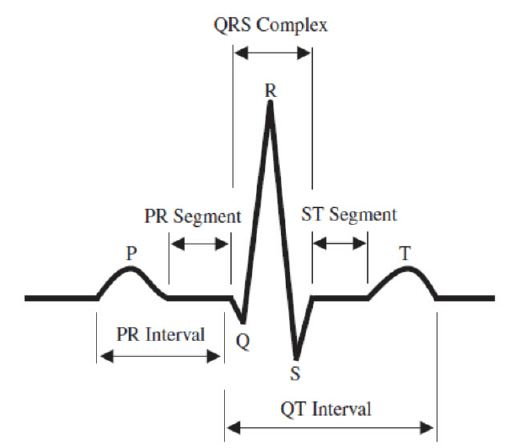
\includegraphics[width=0.4\textwidth]{ecg_components.png}
	\caption{Representation of an ECG signal along with its main components. Source: \cite{ecgcomponents}.}% 
	\label{fig:ecg_components}
\end{figure}

An ECG typically consists of 12 channels known as \emph{leads}, which are derived from electrodes placed on the body in positions that provide different views of the heart. Mathematically however, 8 independent leads are sufficient to convey the full information of a typical ECG, while the other 4 leads can be derived from them \cite{ecgleads}.

\begin{figure}[H]
	\centering
	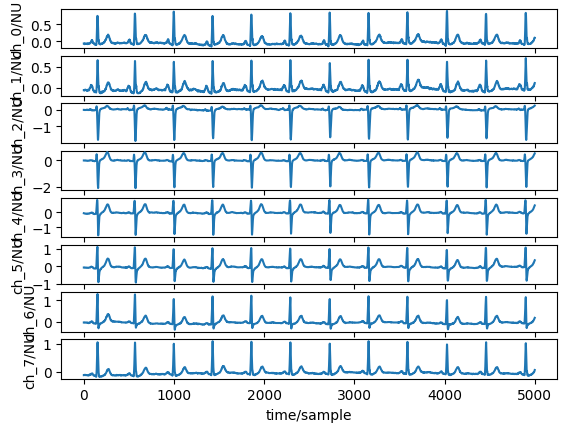
\includegraphics[width=0.7\textwidth]{ecg_example.png}
	\caption{Example of an 8-lead ECG. Source: UMCU dataset (see \refsec{sec:umcu_dataset}).}% 
	\label{fig:ecg_example}
\end{figure}

On the one hand the ECG is easy to produce, but on the other hand it requires expert knowledge in order to be correctly interpreted. This imbalance has a significant negative impact on clinical practice, as there are too many ECGs that need interpretation, and not enough experts to interpret them quickly \cite{ecginterpretation}.

In recent years, efforts have been made to automate the process of ECG interpretation using various algorithms. One of the most urgent issues that diagnostic algorithms have to deal with is noise affecting the signal's interpretability. The main types of noise found in an ECG can be classified as follows \cite{ecgnoisetypes}:
\begin{itemize}
	\item \emph{Baseline wander:} A low-frequency artifact caused by factors like respiration, body movements, and poor electrode contact. It can distort the ST segment and other low-frequency components of the ECG, leading to misdiagnoses of conditions like myocardial infarction.
	\item \emph{Power-line interference:} This type of noise is caused by the coupling of power lines during ECG acquisition, resulting in narrowband noise that can distort ECG morphology, particularly the P wave, potentially leading to incorrect diagnoses of atrial arrhythmias.
	\item \emph{Muscle artifacts} or \emph{electromyogram noise}: Originating from electrical activities in muscles, such as those from movements near the head, these artifacts often overlap with normal ECG frequencies, complicating the recognition of arrhythmias.
	\item \emph{Channel noise:} Induced when ECG signals are transmitted through channels with poor conditions, such as those affected by Additive White Gaussian Noise (AWGN), this type of noise can significantly affect the interpretability of the ECG.
	\item \emph{Composite noise:} A combination of various types of noise.
\end{itemize}
This work aims to apply deep learning techniques in order to detect noisy or otherwise uninterpetable ECGs in an off-line manner, i.e.\ after they have been acquired. ECGs that fall into this category may be considered \emph{Out-of-Distribution} (OOD) in comparison with the interpretable (in-distribution) ECG. Apart from implementing and evaluating traditional OOD detection techniques, we are interested in whether the uncertainty \cite{uncertainty_cordys} in a trained diagnostic classifier's predictions can be used as a measure of noise or unintepretability.

This study was conducted as a part of an internship in association with the company \emph{Cordys analytics}\footnote{\url{https://cordys.health/}}. Any decisions made throughout the experimentation process that require medical knowledge were in consultation with the company's Chief Medical/Technical Officer, Rutger van de Leur\footnote{https://www.researchgate.net/profile/Rutger-Van-De-Leur}, who is a trained cardiologist.

\subsection{Research questions}
\label{sec:research_questions}

Through this work we aim to answer the following research questions:
\begin{customlist}
	\customitem[RQ1]\label{RQ:OOD_detection} What deep learning OOD detection techniques can be used to detect noisy / uninterpretable ECGs before they enter a diagnostic classifier?
	\customitem[RQ2]\label{RQ:noise_vs_abnormal} How can a deep learning model be optimised to distinguish noise from diagnostically important abnormalities in an ECG?
	\customitem[RQ3]\label{RQ:uncertainty} Once an ECG enters a trained diagnostic classifier, can high uncertainty in the classifier's predictions be used to declare the ECG as noisy / uninterpretable?
\end{customlist}


\section{Related work}

Noise detection and/or removal in ECGs has traditionally been done by heuristics \cite{straightforward} or signal processing methods \cite{bayesian,adaptive,ica}. Deep learning techniques appear in the literature for OOD detection in various domains \cite{oodreview}, however to the best of the author's knowledge, not many of them have been applied specifically in the context of off-line detection of noisy ECGs.

Various deep learning methods have been applied to the similar task of anomalous rhythm detection, in works such as \cite{autan,id_ood,abnormal_heart}. While these methods can be attempted also for noise detection, our task differs fundamentally in the following sense: an ECG that is anomalous because it contains an irregular heartbeat is not necessarily noisy, and if labelled as noisy by our pipeline, then it would be a false positive (cf. \ref{RQ:noise_vs_abnormal}).

Specifically in the context of noise detection in ECGs, \cite{binary} introduces a CNN trained on a large private dataset which uses both time and frequency domain information for binary classification of ECGs as ``clean'' or ``noisy'', achieving a ROC-AUC of 0.93. On the other hand, \cite{noise_detection_qrs} uses a CNN to distinguish between ``usable'' and ``unusable'' ECG segments by rejecting those with a level of noise that impacts the accuracy of the QRS complex detection, achieving a ROC-AUC of 0.96. The work \cite{featurespace} applies self-supervised feature extraction and feature-space clustering methods for noise detection without the need of labelled data, achieving varying but generally strong results. Other works such as \cite{denoising1,denoising2,denoising3} focus on denoising ECGs.


\section{Methodology}
\label{sec:methods}

In this work we compare various methods for OOD detection in the domain of ECGs. The methods can be summarised as follows:
\begin{itemize}
	\item \emph{Supervised methods,} which involve training a binary classifier on noise-labelled data in order to classify ECGs as clean or noisy;
	\item \emph{Self-supervised methods,} which include:
	      \begin{itemize}
		      \item training an autoencoder on clean ECGs and using the reconstruction loss as a measure of noise upon testing;
		      \item training a feature-extractor on clean ECGs and using clustering methods on the extracted features of the training data in order to detect outliers upon testing;
	      \end{itemize}
	\item \emph{Uncertainty based methods,} which involve training a classifier for diagnostic purposes on clean ECGs, and using the estimated uncertainty in the classifier's predictions as a measure of noise upon testing.
\end{itemize}

We now explain what each of the above methods entails from a theoretical standpoint. Information about the particular architectures used can be found in \refsec{sec:architectures}, while the implementation and experimentation procedure is detailed in \refsec{sec:exp_and_results}.


\subsection{Binary classification}
\label{sec:bc_method}

The first method we attempt is simple binary classification. In particular, we train a binary classifier
\[
	BC:\, \R^{m\times N} \to \R
\]
on $m$-lead noise-labelled ECGs of length $N$ with the aim to classify ECGs as clean or noisy. The input to the network is an $m$-lead ECG $x$ of length $N$, and the output is a single number $y = BC(x)\in\R$, on which the sigmoid function
\[
	\sigma(y) = \frac{1}{1+e^{-y}}
\]
is applied to obtain the probability of the ECG belonging to the ``noisy'' class. The class of each sample is determined by comparison with a fixed threshold, chosen based on the network's performance on the validation data.


\subsection{Self-supervised methods}

While binary classification is the natural method to use when labelled data is available, the performance of the model greatly depends on the quality of the labels. This can be problematic in the case of outlier detection in general, and more so when applied on signals like ECGs, because labelling itself can be quite hard (see more in \refsec{sec:limitations}). Moreover, large labelled ECG datasets are in general scarce, and can often be found only in a private setting (e.g.\ \cite{binary} as well as this work use a private dataset). While labelled public datasets do exist, they might not always be sufficient for large scale experiments, and artificial data generation is sometimes used to augment the available public datasets (e.g.\ \cite{featurespace} uses synthetic data).

Self-supervised methods provide an alternative way to detect noisy ECGs without the strong reliance on labelled data. In this work we explore two types of self-supervised methods.


\subsubsection{Autoencoder reconstruction loss as a measure of noise}
\label{sec:ae_method}

Similar to \cite{autan}, this method involves training an autoencoder
\[
	AE:\, \R^{m\times N} \to \R^{m\times N}
\]
for the task of reconstruction of clean $m$-lead ECGs of length $N$. Upon testing, the reconstruction loss $\Loss(x, AE(x))$ for a test sample $x$ is calculated. Samples with low/high reconstruction loss are classified as clean/noisy respectively. Classification happens according to a pre-determined threshold based on the pipeline's performance on the validation data.


\subsubsection{Feature space clustering for OOD detection}
\label{sec:fs_method}

Similar to \cite{featurespace}, in this method a neural network
\[
	N = G\circ F :\, \R^{m\times N} \to \R^n
\]
consisting of two parts $F,G$ in sequence, where
\[
	F: \R^{m\times N} \to \R^d \quad \mathrm{and} \quad G: \R^d \to \R^n
\]
(for $d \ll m\times N$) is trained on clean ECGs for a particular task (e.g.\ classification, reconstruction, contrastive learning, etc.). The second part $G$ (which may be a classification head, a decoder, etc.) is then discarded, and the first part $F$ is used as a feature extractor, i.e.\ a mapping into the lower dimensional space $\R^d$ which maintains important information about the input. After training, the features extracted from the training set $X_{train}$ are clustered using a \emph{Gaussian Mixture Model (GMM)}. Given a test sample $x$, the minimum \emph{Mahalanobis distance} between $F(x)$ and the training feature clusters is calculated. Samples with low/high Mahalanobis distance are classified as clean/noisy respectively.

In this work, the following tasks were used to obtain feature extractors:
\begin{itemize}
	\item An autoencoder was trained for reconstruction of clean ECGs. The encoder part was then used as a feature extractor.
	\item A classifier was trained on various diagnostic labels. The classification head was then removed and the rest of the network was used as a feature extractor.
	\item Contrastive learning (SimCLR) was used to directly learn feature representations.
\end{itemize}

We now briefly explain some of the technical terms introduced in this section.

\paragraph{Gaussian Mixture Model.} A GMM is a probabilistic model which assumes that all data-points are generated from a finite number of possibly correlated Gaussian distributions. Popular algorithms that fit GMMs to data (such as the one in \texttt{scikit-learn}, which was used in this work) try to estimate the parameters of each cluster and the interaction between the clusters using an expectation-maximization algorithm \cite{gmm}.

\paragraph{Mahalanobis distance.} The Mahalanobis distance \cite{mahalanobis} is a measure of distance between a point and a distribution. Given a point $x\in\R^d$ and a distribution $D$ over $\R^d$ with mean $\mu$ and covariance $\Sigma$, the Mahalanobis distance between $x$ and $D$ is given by:
\[
	M(x, D) = \sqrt{(x-\mu)^T\Sigma^{-1}(x-\mu)}
\]
Under the assumption that $D$ is Gaussian, $M$ can be shown to follow the chi-squared distribution with $d$ degrees of freedom. As a result, the CDF of the chi-squared distribution can be used to determine outliers at a certain confidence threshold of our choice. Since however $D$ being Gaussian is generally too strict of an assumption, the threshold can also be chosen once again empirically.

\paragraph{SimCLR.} SimCLR \cite{simclr} is a self-supervised framework for contrastive learning of low-dimensional representations of a dataset. The framework works as follows:
\begin{enumerate}
	\item During each epoch, two (or more) random augmentations are produced for each data-point in a training batch.
	\item The augmented samples are embedded through the feature extractor $F$ (often an additional projection head $G$ is added after $F$) into a low dimensional feature space.
	\item For each batch, the InfoNCE loss \cite{infonce} is calculated. In short, the InfoNCE loss tries to minimise the cosine similarity between augmentations of the same sample, and maximize that between augmentations of different samples.
	\item After training, $F$ is used as a feature extractor.
\end{enumerate}


\subsection{Uncertainty based methods}
\label{sec:un_method}

It has been observed that DNNs can produce incorrect predictions with high confidence on OOD data \cite{calibration}. To counter this, various methods have been developed in order to estimate the \emph{uncertainty} associated with a DNN's predictions. Uncertainty can be a result of two causes:
\begin{itemize}
	\item \emph{Aleatoric uncertainty} arises from the inherent randomness in data, which can be background noise, measurement errors, or inconsistencies that can't be eliminated by gathering more data.
	\item \emph{Epistemic uncertainty} is due to the model's lack of experience with data-points outside its training, and can be reduced by providing the model with more diverse data points that better represents the domain distribution.
\end{itemize}
In a medical setting, uncertainty estimation is crucial in order to avoid confident but erroneous predictions from an automated diagnostic system. The comprehensive study \cite{uncertainty_cordys} investigates various estimation techniques for both types of uncertainty in the context of ECG classification. Works such as \cite{uncertainty_ood} also suggest that uncertainty estimation can be used for OOD detection.

In the context of ECG noise detection, the hypothesis explored in this work is that given a variety of training data, any sample which is determined to be OOD compared to them through uncertainty-based methods may be considered noisy, or unsuitable for diagnostic purposes (\ref{RQ:uncertainty}). The method is implemented as follows. A classifier
\[
	C:\, \R^{m\times N} \to \R^n
\]
is trained on clean $m$-lead ECGs for prediction of various diagnostic labels. Upon testing, the (epistemic) uncertainty of the model's predictions is estimated. Samples with low/high uncertainty scores are classified as clean/noisy respectively, by comparison to a chosen threshold. The methods used to estimate uncertainty in this work are the following:
\begin{itemize}
	\item \emph{Ensemble methods,} which involve training the same architecture a number of times using different weight initializations, resulting in an ensemble of networks. The variance in the ensemble's predictions for any given input can be used as a measure of (epistemic) uncertainty \cite{uncertainty_cordys}.
	\item \emph{Monte-Carlo dropout methods,} which apply on any network that is trained using dropout. Dropout is also kept upon testing, thus masking different weights of the network every time a prediction is made. The variance in the network's predictions for the same input over different dropout masks can be used as a measure of (epistemic) uncertainty \cite{uncertainty_cordys}.
\end{itemize}


\subsection{Evaluation metrics}

All of our models output a value which is to be compared with a threshold in order to make a classification decision. In order to assess the ability of our models to distinguish between the positive and the negative class over all classification thresholds, we use the ROC-AUC score, which stands for \textbf{R}eceiver \textbf{O}perating \textbf{C}haracteristic - \textbf{A}rea \textbf{U}nder \textbf{C}urve. The ROC curve is the plot of the True Positive rate (TPR) against the False Positive rate (FPR) at each distinct classification threshold, and its area is equal to the probability that the classifier ranks a randomly chosen positive example higher than a randomly chosen negative example \cite{roc}. A perfect classifier receives a ROC-AUC score of 1, whereas a random classifier receives a score of 0.5. The ROC-AUC score is a standard metric often used in medical settings for comparing different diagnostic tests and determining their overall diagnostic performance \cite{rocmedicine}.

Suppose now that for a specific model the threshold is chosen to produce a classifier which makes predictions $\hat{y}$ for each input $x$ with true label $y$. We are interested in the following metrics:
\begin{itemize}
	\item \emph{True Positive rate} (TPR), aka \emph{sensitivity}, or \emph{recall}:
	      \[
		      P(\hat{y} = 1 \,|\, y = 1) = \frac{TP}{TP + FN}
	      \]
	\item \emph{True Negative rate} (TNR), aka \emph{specificity}:
	      \[
		      P(\hat{y} = 0 \,|\, y = 0) = \frac{TN}{TN + FP}
	      \]
	\item \emph{False Positive rate} (FPR), i.e.\ 1 - specificity:
	      \[
		      P(\hat{y} = 1 \,|\, y = 0) = \frac{FP}{TN + FP}
	      \]
	\item \emph{False Negative rate} (FNR), i.e.\ 1 - sensitivity:
	      \[
		      P(\hat{y} = 0 \,|\, y = 1) = \frac{FN}{TP + FN}
	      \]
\end{itemize}
The above metrics are reported by means of confusion matrices, the rows of which are normalised by the number of samples with positive true label:
\begin{table}[H]
	\centering
	\begin{tabular}{c|c}
		TNR & FPR \\\midrule
		FNR & TPR
	\end{tabular}
\end{table}

We are also interested in other standard classification metrics:
\begin{itemize}
	\item \emph{Accuracy}:
	      \[
		      P(\hat{y} = y) = \frac{TP + TN}{TP + TN + FP + FN}
	      \]
	\item \emph{Precision}:
	      \[
		      P(y = 1 \,|\, \hat{y} = 1) = \frac{TP}{TP + FP}
	      \]
	\item \emph{F1 score}:
	      \[
		      2 \cdot \frac{\text{Precision} \cdot \text{Recall}}{\text{Precision} + \text{Recall}}
	      \]
\end{itemize}

Any confidence intervals (CI) reported on the metrics are calculated by bootstrapping \cite{bootstrap} on the test set.

\section{Datasets}

In this work we use 8-lead ECGs of length 5,000 for training and testing our algorithms. We mainly use two datasets, one of which is private, while the other is public.

\subsection{UMCU dataset}
\label{sec:umcu_dataset}

Our private dataset is provided by Cordys Analytics in collaboration with the University Medical Center Utrecht (UMCU)\footnote{\url{https://www.umcutrecht.nl/en}}. The dataset consists of 386,413 8-lead ECGs sampled at 500 Hz over 10 seconds. This dataset is labelled by a panel of experts on more than 100 diagnostic criteria, including on existence of noise, and is the main dataset used for training, validation and testing.
\subsubsection{Noise label}

The UMCU dataset contains two noise labels:
\begin{itemize}
	\item \emph{quality\_to} (technisch onvolwaardig - technically defective), which indicates the presence of morphological noise in the ECG, such as significant baseline wander, high-frequency noise, missing leads, or other signal interference. This type of noise can be caused by many reasons including power line interference, muscle artefacts, movement of the patient, poor electrical connection, or other external sources.
	\item \emph{quality\_tf} (technische fout - technical error), which indicates that the order of leads in the ECG is incorrect. This type of noise is normally caused by misplaced electrodes during testing.
\end{itemize}

Both labels include different levels of noise (0-3 for quality\_to, 0-2 for quality\_tf). However, fewer than 0.01\% of the total samples were found to have labels of level greater than 1. Therefore we opt for a binary label system instead, with 1 indicating any level of noise and 0 indicating lack of noise. The resulting label distributions are:
\begin{table}[H]
	\parbox{0.45\linewidth}{
		\raggedleft
		\begin{tabular}{r|l}
			\multicolumn{2}{c}{\textbf{quality\_to}} \\\midrule
			0 & 373,452                              \\
			1 & 12,961                               \\
		\end{tabular}
	}
	\hfill
	\parbox{0.45\linewidth}{
		\raggedright
		\begin{tabular}{r|l}
			\multicolumn{2}{c}{\textbf{quality\_tf}} \\\midrule
			0 & 385,607                              \\
			1 & 806                                  \\
		\end{tabular}
	}
\end{table}

A sample in which either label is positive is labelled as ``noisy''. The resulting \emph{Noise} label has the following distribution:
\begin{table}[H]
	\centering
	\begin{tabular}{r|l}
		\multicolumn{2}{c}{\textbf{Noise}} \\\midrule
		0 & 372,761                        \\
		1 & 13,652                         \\
	\end{tabular}
\end{table}

\Cref{fig:umcu_noise_labels} presents randomly selected examples of ECGs with different noise labels from the UMCU dataset.
\begin{figure}[htbp]
	\centering
	\makebox[\linewidth][c]{
		\begin{subfigure}[b]{0.6\textwidth}
			\centering
			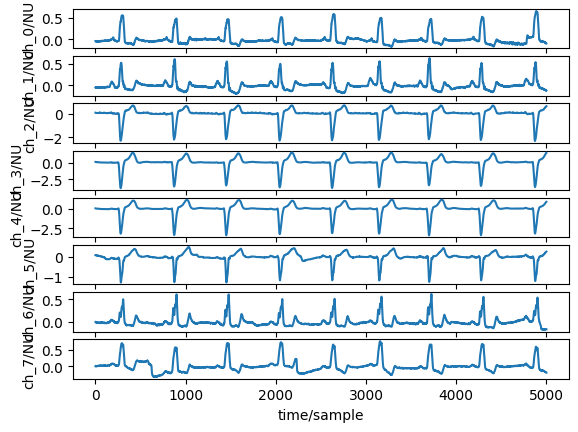
\includegraphics[width=\textwidth]{quality_to=0-quality_tf=0.png}
			\caption{quality\_to = 0, quality\_tf = 0 (clean)}% 
			\label{fig:qto0_qtf0}
		\end{subfigure}%
		\begin{subfigure}[b]{0.6\textwidth}
			\centering
			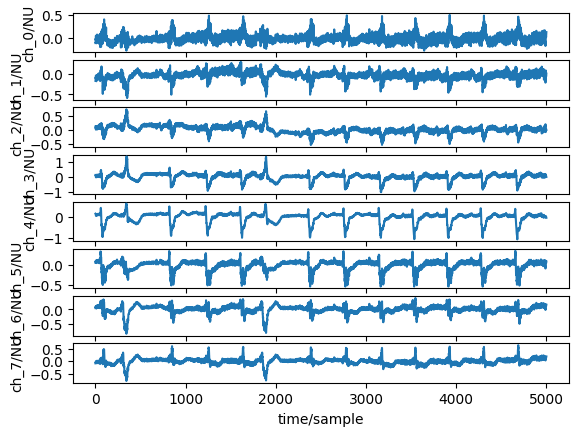
\includegraphics[width=\textwidth]{quality_to=1-quality_tf=0.png}
			\caption{quality\_to = 1, quality\_tf = 0 (noisy)}% 
			\label{fig:qto1_qtf0}
		\end{subfigure}
	}
	\vskip\baselineskip
	\makebox[\linewidth][c]{
		\begin{subfigure}[b]{0.6\textwidth}
			\centering
			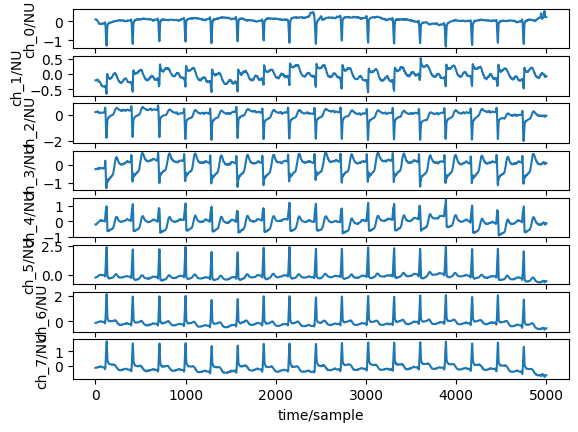
\includegraphics[width=\textwidth]{quality_to=0-quality_tf=1.png}
			\caption{quality\_to = 0, quality\_tf = 1 (noisy)}% 
			\label{fig:qto0_qtf1}
		\end{subfigure}%
		\begin{subfigure}[b]{0.6\textwidth}
			\centering
			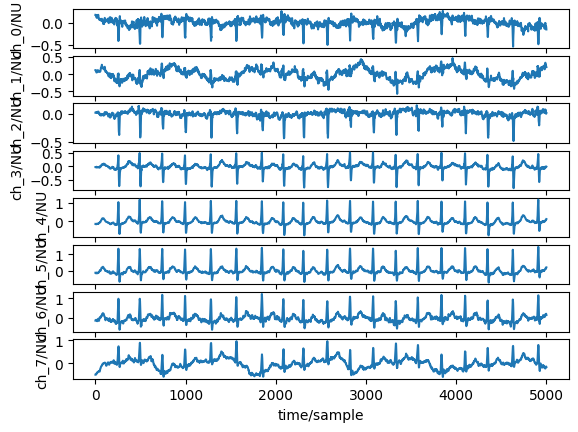
\includegraphics[width=\textwidth]{quality_to=1-quality_tf=1.png}
			\caption{quality\_to = 1, quality\_tf = 1 (noisy)}% 
			\label{fig:qto1_qtf1}
		\end{subfigure}
	}
	\caption{Examples of ECGs from the UMCU dataset with different noise labels.}
	\label{fig:umcu_noise_labels}
\end{figure}


\subsubsection{Expert-annotated set}

During the internship, a panel of experts in collaboration with Cordys Analytics further labelled a subset of 992 UMCU ECGs. The new labels are deemed to be of higher quality than those available before, and contain detailed annotations about how each ECG should be segmented into its distinct components, while also including noisy segments. Due to the fact that the main algorithms and pipelines had already been developed by the time that the new annotations became available to the author, the segmentation information was not used (see more in \refsec{sec:limitations}). Instead, for the purposes of this work, every ECG which contained noise annotations was classified as noisy, resulting in the following distribution:
\begin{itemize}
	\item 976 clean ECGs;
	\item 16 noisy ECGs.
\end{itemize}
This subset is used for testing purposes.


\subsection{PhysioNet 2011 dataset}

The PhysioNet 2011 Challenge \cite{physionet2011paper,goldberger2000physiobank} aimed to create an efficient algorithm that can quickly provide feedback regarding the diagnostic interpretability of ECGs recorded in any setting, possibly by a non-expert. The public dataset associated with the challenge can be downloaded from \cite{physionet2011dataset}. It contains 1,000 noise-labelled 12-lead ECG recordings sampled at 500 Hz over 10 seconds, which were made by various experts and non-experts. The samples were reviewed by a group of independent annotators with various degrees of expertise, and the average label was calculated. The quality of 2 samples is labelled as ``undetermined'' due to lack of agreement between the annotators, while the other 998 ECGs have the following label distribution:
\begin{itemize}
	\item 773 ``acceptable'' (clean);
	\item 225 ``unacceptable'' (noisy).
\end{itemize}
The 998 ECGs with unambiguous labels are used in this work for testing purposes. \Cref{fig:phynet_noise_labels} shows randomly selected examples of clean and noisy ECGs from the PhysioNet 2011 dataset.
\begin{figure}[htbp]
	\centering
	\makebox[\linewidth][c]{
		\begin{subfigure}[b]{0.6\textwidth}
			\centering
			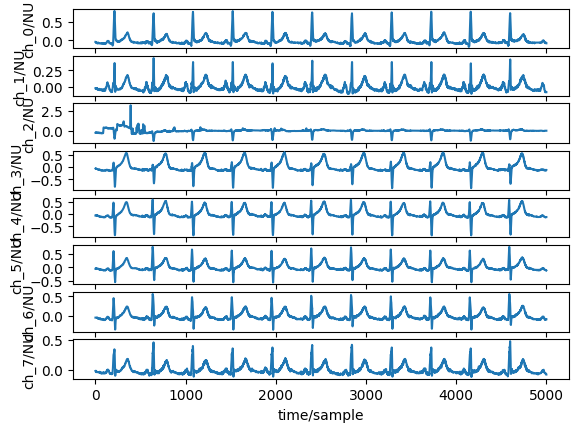
\includegraphics[width=\textwidth]{phynet_noise=0.png}
			\caption{PhysioNet 2011 dataset, clean example}% 
			\label{fig:phynet_noise-0}
		\end{subfigure}%
		\begin{subfigure}[b]{0.6\textwidth}
			\centering
			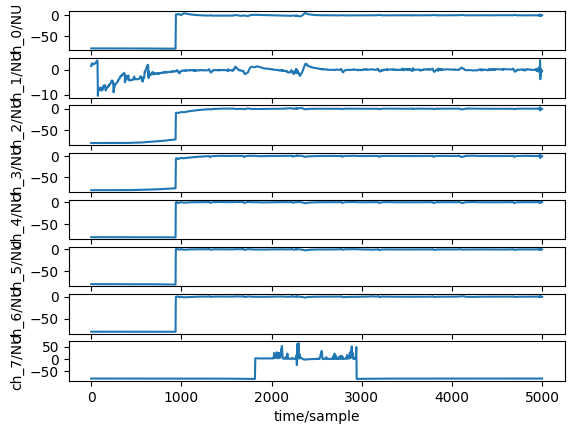
\includegraphics[width=\textwidth]{phynet_noise=1.png}
			\caption{PhysioNet 2011 dataset, noisy example}% 
			\label{fig:phynet_noise-1}
		\end{subfigure}
	}
	\caption{Examples of ECGs from the PhysioNet 2011 dataset with different noise labels.}
	\label{fig:phynet_noise_labels}
\end{figure}


\section{Data preprocessing}

We now explain the preprocessing that was applied on the data. First, we discuss the issue of data normalisation.


\subsection{Data normalisation}
\label{sec:data_normalisation}

When training a DNN for example in computer vision, it is typical to normalise the data so that all the values are in the range $[0, 1]$ or $[-1, 1]$. This is not advisable in the case of ECGs for the following reasons:
\begin{itemize}
	\item The scale of an ECG has a diagnostic meaning, i.e.\ different conditions can produce heart rhythms of different amplitudes. Therefore, any model used for diagnostic purposes must take the scale of an ECG into account.
	\item Noise in the signal is also scale-dependent, and normalising the values of the ECG would also normalise the noise. This is undesirable for types of noise that may present with amplitudes outside the normal ECG range, such as large baseline drift. On the other hand, if the ECG contains Gaussian noise with small amplitude, then normalisation would make this noise harder to detect. The above points are particularly relevant for the reconstruction experiments, where normalising the noise would lead to better reconstructions of noise itself, leading to an increase of FNR (see \refsec{sec:ae_exp}).
\end{itemize}
Instead of normalisation, the gain value of 0.00488 was applied on each signal in order to convert it from the scale in which it was stored in the dataset, which is of order $\mu$Volt ($\mu$V), to the order of mVolt (mV). The value itself is obtained from the dataset's metadata, and indicates an average gain value that should be appropriate for the vast majority of the ECGs in it (since individual gain values are not stored). Thus, most ECG signals in the dataset end up being within the range of $[-5, 5]$ (in mV), which is normal for ECGs \cite{ecgstats}. More on the statistical distribution of the clean signals of the UMCU dataset in particular is analysed in \refsec{sec:clean_split_a}.


\subsection{UMCU data}

The UMCU data is split in three ways for the different experiments.


\subsubsection{Binary classification split}
\label{sec:binary_split}

For the binary classification experiments, the data is split into train/validation/test sets, with relative sizes 0.8/0.1/0.1. The split is performed at the patient ID level, in order to avoid ECGs from the same patient to end up in different sets.


\subsubsection{Clean split A}
\label{sec:clean_split_a}

For the rest of the experiments we aim to use only clean ECGs for training, hence the noisy ECGs are all removed from the training set. Additionally, we want to remove ECGs with morphological properties that possibly indicate noise, but can be easily detected by a rule-based system. Therefore, ECGs are additionally removed if:
\begin{itemize}
	\item The \emph{maximum absolute value} in the ECG (after applying gain) is greater than 5 (3,264 ECGs are flagged).
	\item The \emph{maximum standard deviation} over all leads of the ECG (after applying gain) is greater than 1 (4,675 ECGs are flagged).
	\item The \emph{minimum standard deviation} over all leads of the ECG (after applying gain) is less than 0.02 (560 ECGs are flagged).
\end{itemize}
Note that the above rules may overlap. In total, along with the 13,652 noisy ECGs, another 5,564 ECGs are removed to make a total of 19,216 OOD ECGs, leaving a set of 367,197 in-distribution ECGs. Once again, the data is split into train/validation/test sets at the patient ID level, with relative sizes 0.8/0.1/0.1.

\Cref{fig:stats_ood} shows examples of ECGs that are removed by our rule-based filters, but are not labelled as noisy.
\begin{figure}[htbp]
	\centering
	\makebox[\linewidth][c]{
		\begin{subfigure}[b]{0.6\textwidth}
			\centering
			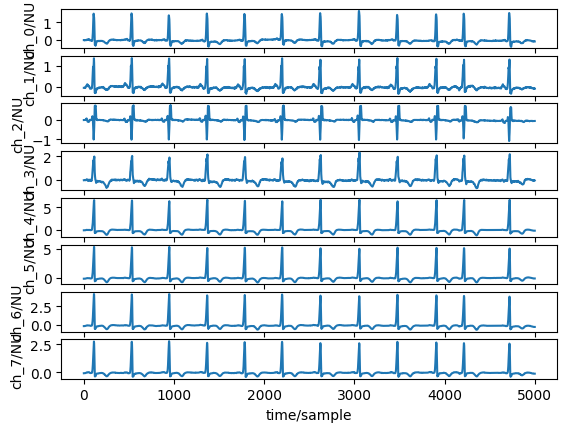
\includegraphics[width=\textwidth]{max_abs5.png}
			\caption{Max abs. value $> 5$, noise label = 0}% 
			\label{fig:max_abs5}
		\end{subfigure}%
		\begin{subfigure}[b]{0.6\textwidth}
			\centering
			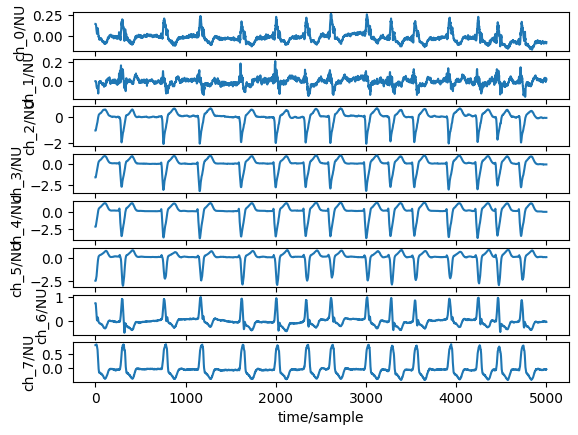
\includegraphics[width=\textwidth]{max_sd1.png}
			\caption{Max SD $> 1$, noise label = 0}% 
			\label{fig:max_sd1}
		\end{subfigure}
	}
	\vskip\baselineskip
	\begin{subfigure}[b]{0.6\textwidth}
		\centering
		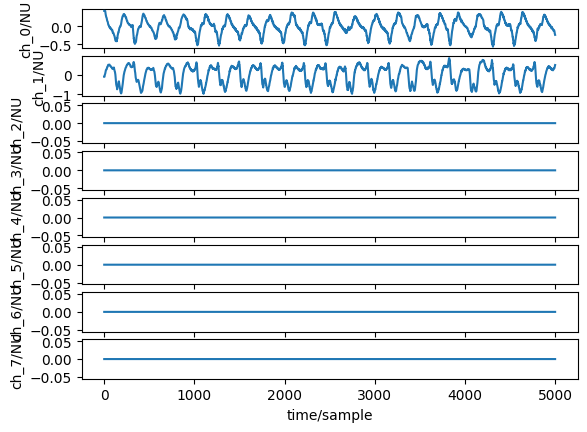
\includegraphics[width=\textwidth]{min_sd002.png}
		\caption{Min SD $< 0.02$, noise label = 0}% 
		\label{fig:min_sd002}
	\end{subfigure}
	\caption{Examples of ECGs that are labelled as clean but are flagged as OOD by our filters.}
	\label{fig:stats_ood}
\end{figure}

\paragraph{Noise detection test set.} Out of the 13,652 noisy ECGs, we discard 1,040 ECGs that are easily flagged by the above rules, and we are left with 12,612 noisy ECGs. Along with the in-distribution test set, which consists of 36,593 clean ECGs, we form a set of 49,205 ECGs on which the reconstruction and the feature space methods are tested for ECG noise detection. Note that the ECGs that were removed based on morphological properties are not included in the noise detection test set, since they can be detected anytime by the same simple rules.


\subsubsection{Clean split B}
\label{sec:clean_split_b}

For the uncertainty based experiments, along with noisy ECGs we also aim to detect ``difficult'' ECGs, which are either rare in real-world scenarios, or challenging even for human experts to interpret. We would also like to evaluate our algorithms on a test set that does not contain such difficult examples in the clean label. For the above purposes, we use the diagnostic labels available in the UMCU dataset to determine the following categories of interest:
\begin{itemize}
	\item \emph{Rhythm type:} 12 mutually exclusive labels (multi-class);
	\item \emph{AV conduction:} 4 mutually exclusive labels (multi-class);
	\item \emph{Ventricular conduction:} 4 mutually exclusive labels (multi-class);
	\item \emph{Ischemia:} 3 mutually exclusive labels (multi-class);
	\item \emph{Other:} 6 independent labels (multi-label).
\end{itemize}
While it is not impossible in a real life clinical scenario for some labels to co-exist in the above multi-class categories, it is quite rare for this to happen, and might be indicative of severe pathology, or of an ECG that is hard to interpret. Our hypothesis is that such ECGs should result in increased uncertainty in a diagnostic model's predictions. To test this hypothesis, out of the 367,197 ECGs of Clean split A, we keep only those that are labelled with a single class in the multi-class categories. In total, 18,543 more ECGs are removed in this manner, leaving a set of 348,654 in-distribution ECGs. Train/validation/test splits are constructed by filtering the corresponding splits of Clean split A. The corresponding noise detection test set is constructed by combining the 12,612 noisy ECGs that are left behind by Clean split A, along with the 35,097 ECGs that are left in the test set of Clean split B after filtering the test set of Clean split A. Note that we do not further filter the noisy part of the noide detection test set through the diagnostic rules, since detecting noise by first figuring out the diagnostic labels defeats the purpose.

\subsubsection{Expert-annotated set}

The expert annotated-set is ensured to be entirely contained within the test sets of all the other UMC splits. After filtering this set with the morphological rules of \refsec{sec:clean_split_a}, we are left with 976 ECGs that pass our filters, out of which:
\begin{itemize}
	\item 962 are clean;
	\item 14 are noisy.
\end{itemize}


\subsection{PhysioNet 2011 data}
\label{sec:physionet_stats}

The PhysioNet 2011 is used exclusively for testing. After removing outliers based on our morphological rules, only 299 ECGs remain, out of which:
\begin{itemize}
	\item 276 are clean;
	\item 23 are noisy.
\end{itemize}
While a lot of ECGs that are labelled as clean are excluded, this is justified since it is important to keep a consistent distribution across all test sets.


\subsection{Summary of data splits}

This section summarises the information about the different datasets, their usage, the manner in which they were split during experimentation, and their label distribution.

\paragraph{Usage of each split.} \Cref{tab:data-splits-usage} shows how each split is used in the different methods tested in this work.
\begin{table}[htbp]
	\begin{tabular}{r|c|c|c|c}
		                       & \textbf{Binary class.}    & \textbf{Reconstruction}   & \textbf{Feature space}    & \textbf{Uncertainty}      \\ \midrule
		\textbf{Binary class.} & \textbf{train, val, test} & \emph{n/a}                & \emph{n/a}                & \emph{n/a}                \\
		\textbf{Clean split A} & \emph{n/a}                & \textbf{train, val, test} & \textbf{train, val, test} & \emph{n/a}                \\
		\textbf{Clean split B} & \emph{n/a}                & test                      & test                      & \textbf{train, val, test} \\
		\textbf{Expert-ann.}   & test                      & test                      & test                      & test                      \\
		\textbf{PhysioNet}     & test                      & test                      & test                      & test
	\end{tabular}
	\caption{Usage of each split.}
	\label{tab:data-splits-usage}
\end{table}

\paragraph{Binary classification split.} \Cref{tab:binary-data-split} shows the label distribution over all splits used for training and evaluation of the binary classification algorithm.
\begin{table}[htbp]
	\centering
	\begin{tabular}{r|c|c|c|c}
		               & \textbf{Training set} & \textbf{Validation set} & \textbf{Test set} & \textbf{Sum} \\ \midrule
		\textbf{Clean} & 298,865               & 36,827                  & 37,069            & 372,761      \\
		\textbf{Noisy} & 10,952                & 1,360                   & 1,340             & 13,652       \\ \midrule
		\textbf{Sum}   & 309,817               & 38,187                  & 38,409            & 386,413
	\end{tabular}
	\caption{Summary of binary classification data split.}
	\label{tab:binary-data-split}
\end{table}

\paragraph{Clean splits.} \Cref{tab:clean-split-a-dist} summarises how the data is split in order to form Clean split A according to the chosen morphological rules.
\begin{table}[htbp]
	\centering
	\begin{tabular}{r|c|c|c}
		\textbf{Clean split A} & \textbf{Pass rules} & \textbf{Fail rules} & \textbf{Sum} \\ \midrule
		\textbf{Clean}         & 367,197             & 5,564               & 372,761      \\
		\textbf{Noisy}         & 12,612              & 1,040               & 13,652       \\ \midrule
		\textbf{Sum}           & 379,807             & 6,604               & 386,413
	\end{tabular}
	\caption{Construction of Clean split A.}
	\label{tab:clean-split-a-dist}
\end{table}

Now each sub-split of Clean split B is simply a subset of the corresponding sub-split of Clean split A that was filtered using the diagnostic rules. The noisy ECGs are not subject to the diagnostic rules. \Cref{tab:clean-split-b-dist} shows how Clean split B is formed according to the morphological as well as the diagnostic rules.
\begin{table}[htbp]
	\centering
	\begin{tabular}{r|c|c|c}
		\textbf{Clean split B} & \textbf{Pass rules} & \textbf{Fail rules} & \textbf{Sum} \\ \midrule
		\textbf{Clean}         & 348,654             & 24,107              & 372,761      \\
		\textbf{Noisy}         & 12,612              & 1,040               & 13,652       \\ \midrule
		\textbf{Sum}           & 361,266             & 25,147              & 386,413
	\end{tabular}
	\caption{Construction of Clean split B.}
	\label{tab:clean-split-b-dist}
\end{table}

\Cref{tab:clean-train-val-test} summarises how Clean split A and Clean split B are used for training and testing. Here, \emph{training} refers to the actual training set, \emph{validation} refers to the set used for validation during training in order to select the best model, and \emph{testing} refers to the set kept aside to be used along with the noisy data for evaluation of the algorithms on noise detection.

\begin{table}[htbp]
	\centering
	\begin{tabular}{r|c|c}
		                    & \textbf{Clean split A} & \textbf{Clean split B} \\ \midrule
		\textbf{Training}   & 294,046                & 278,719                \\
		\textbf{Validation} & 36,558                 & 34,838                 \\
		\textbf{Testing}    & 36,593                 & 35,097                 \\ \midrule
		\textbf{Sum}        & 367,197                & 348,654
	\end{tabular}
	\caption{Summary of data that is used for training/testing purposes on each split.}
	\label{tab:clean-train-val-test}
\end{table}

\paragraph{Noise detection test sets.} \Cref{tab:all-noise-test} shows the label distribution of all the sets that are used for testing our algorithms on the task of noise detection.

\begin{table}[htbp]
	\centering
	\begin{tabular}{r|c|c|c|c|c}
		               & \textbf{Binary class.} & \textbf{Clean A} & \textbf{Clean B} & \textbf{Expert-ann.} & \textbf{PhysioNet 2011} \\ \midrule
		\textbf{Clean} & 37,069                 & 36,593           & 35,097           & 962                  & 276                     \\
		\textbf{Noisy} & 1,340                  & 12,612           & 12,612           & 14                   & 23                      \\ \midrule
		\textbf{Sum}   & 38,409                 & 49,205           & 47,709           & 976                  & 299
	\end{tabular}
	\caption{Summary of sets that are used for testing the noise detection algorithms.}
	\label{tab:all-noise-test}
\end{table}

\section{Architectures}
\label{sec:architectures}

In total, 4 different model architectures are used during the experimentation process:
\begin{enumerate}
	\item a \emph{binary classifier} (BinCl);
	\item an \emph{autoencoder} (AE);
	\item a \emph{diagnostic classifier} (DiagCl);
	\item a \emph{SimCLR} architecture.
\end{enumerate}
In this section we go into details about each architecture.

\subsection{Binary classifier}
\label{sec:bincl_architecture}

The main BinCl architecture consists of a double residual 1-D convolutional encoder, based on \cite{doubleresidual}, followed by a classification head. Dropout layers are used both in the encoder as well as before the classifier, while non-linearity is added to the classification head by means of the RELU activation function. An example of the architecture can be found in \Cref{fig:bincl_architecture}.
\begin{figure}[htbp]
	\centering
	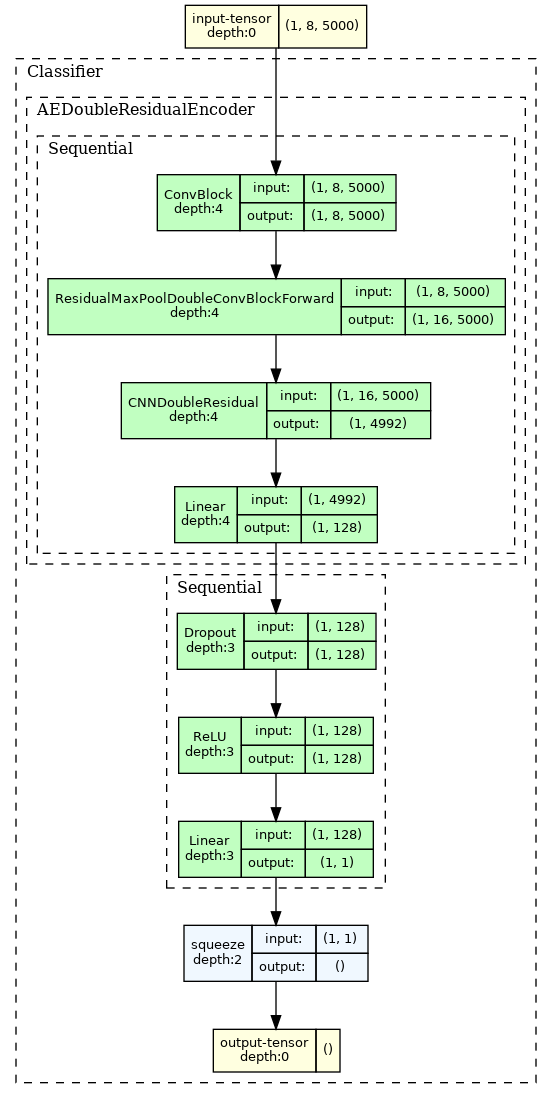
\includegraphics[width=0.7\textwidth]{Binary_Classifier.gv.png}
	\caption{Binary classifier architecture.}% 
	\label{fig:bincl_architecture}
\end{figure}
More detailed views of the components of the encoder can be found in \refsec{sec:appendix}, \Cref{fig:convblock_architecture,fig:resbw_architecture,fig:cnnfw_architecture}.

\subsection{Autoencoder}
\label{sec:ae_architecture}

The main AE architecture used for our experiments consists of a double residual encoder and a double residual decoder, based on \cite{doubleresidual}. \Cref{fig:ae_architecture} shows an example of the architecture.
\begin{figure}[htbp]
	\centering
	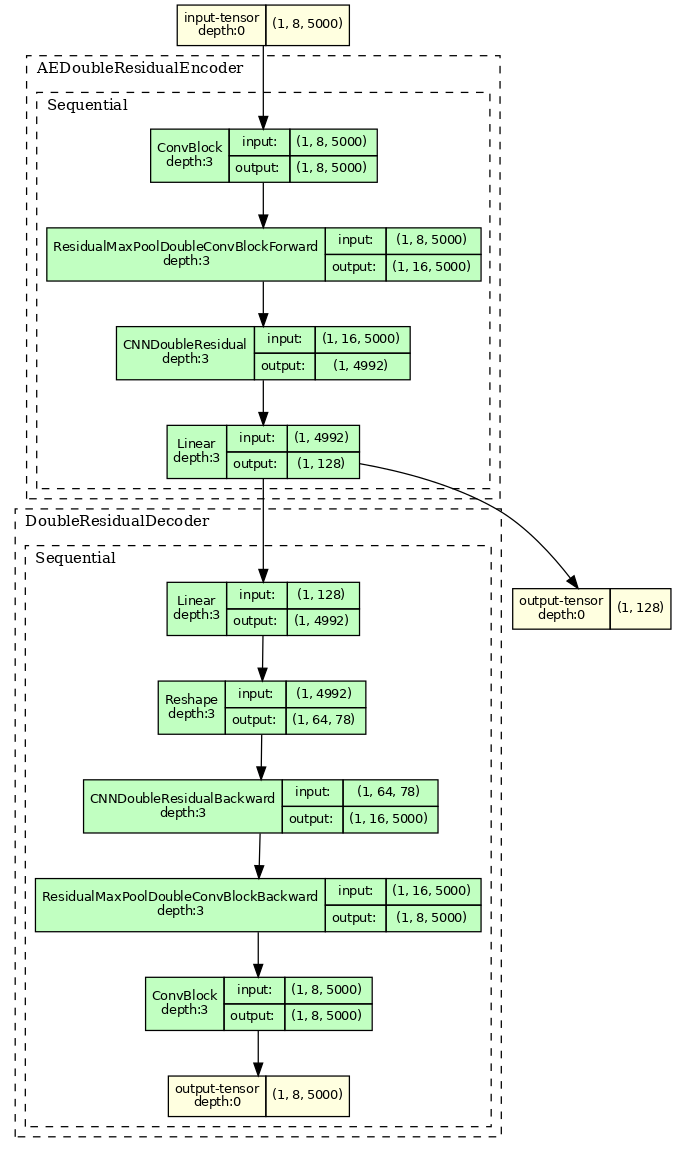
\includegraphics[width=0.85\textwidth]{AE.gv.png}
	\caption{AE architecture.}% 
	\label{fig:ae_architecture}
\end{figure}
The decoder architecture mirrors the one of the encoder (see \refsec{sec:bc_exp}), containing the same components but in a reverse order. The architectures of the mirrored components can be seen in \refsec{sec:appendix}, \Cref{fig:resbw_architecture,fig:cnnbw_architecture}.



\subsection{Diagnostic classifier}
\label{sec:diagcl_architecture}

The DiagCl architecture consists of a double residual encoder \cite{doubleresidual}, along with 5 independent classification heads, one for each diagnostic class of interest as defined in \refsec{sec:clean_split_b}. Each classification head consists of a dropout layer followed by RELU and a linear layer. \Cref{fig:diagcl_architecture} shows an example of the architecture of the DiagCl model.
\begin{figure}[htbp]
	\centering
	\makebox[\textwidth][c]{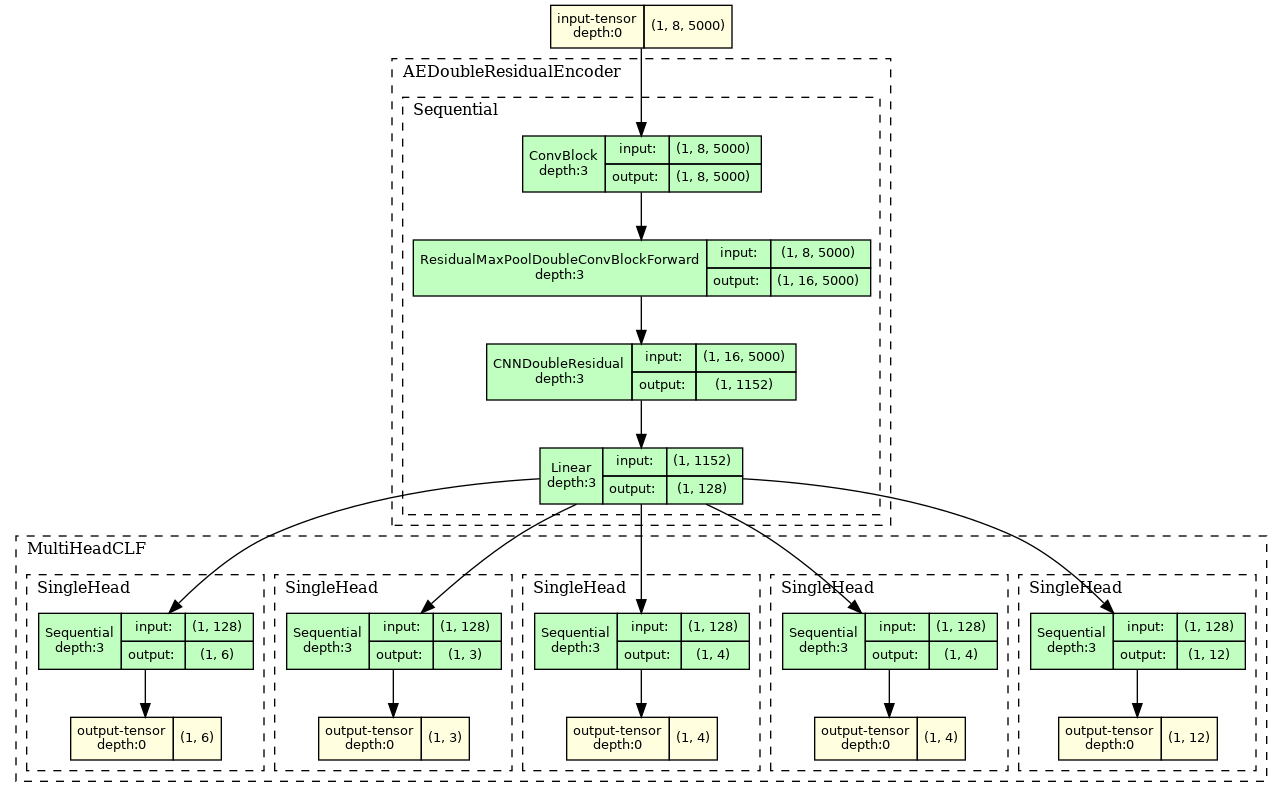
\includegraphics[width=1.3\textwidth]{MultiClassifier.gv.png}}%
	\caption{DiagCl architecture.}% 
	\label{fig:diagcl_architecture}
\end{figure}


\subsection{SimCLR}
\label{sec:simclr_architecture}

Our implementation of the SimCLR architecture consists of a double residual encoder \cite{doubleresidual} followed by a projection head. The use of projection heads in contrastive learning is studied extensively in \cite{simclrprojection}, where it is shown that using a non-linear projection head during training, and then discarding it in order to obtain embeddings from the layer just before it, produces better representations compared to training by applying the InfoNCE loss on the feature extractor directly.
\begin{figure}[htbp]
	\centering
	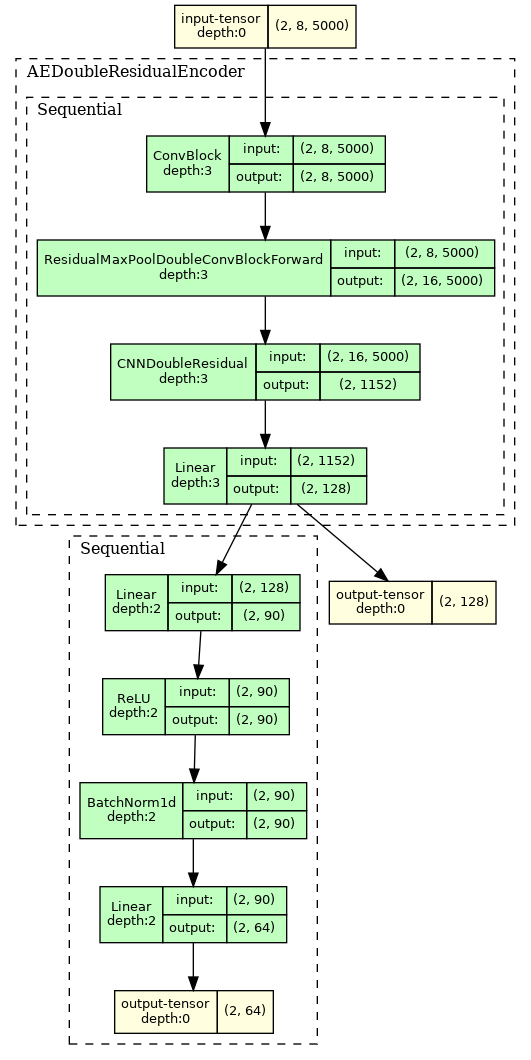
\includegraphics[width=0.7\textwidth]{SimCLR.gv.png}
	\caption{SimCLR architecture.}% 
	\label{fig:simclr_architecture}
\end{figure}


\subsection{Summary of models and methods}

Each method uses specific architectures as its main tools. However, some architectures may be used as secondary tools during the experiments of each method in order to assist training, e.g.\ for better weight initialization. \Cref{tab:models-sum} shows a summary of which models were used for which method. Details about how each model was used can be found in \refsec{sec:exp_and_results}.

\begin{table}[htbp]
	\begin{tabular}{r|c|c|c|c}
		                           & \textbf{Binary class.} & \textbf{Reconstruction} & \textbf{Feature space} & \textbf{Uncertainty} \\ \midrule
		\textbf{Binary class.}     & \textbf{main}          & \emph{n/a}              & \emph{n/a}             & \emph{n/a}           \\
		\textbf{Autoencoder}       & \emph{n/a}             & \textbf{main}           & \textbf{main}          & \emph{n/a}           \\
		\textbf{Diagnostic class.} & \emph{n/a}             & secondary               & \textbf{main}          & \textbf{main}        \\
		\textbf{SimCLR}            & \emph{n/a}             & secondary               & \textbf{main}          & secondary
	\end{tabular}
	\caption{Summary of models and methods in which they were used}
	\label{tab:models-sum}
\end{table}


\section{Experiments and Results}
\label{sec:exp_and_results}

We now go into details about the experiments conducted with each of the methods described in \refsec{sec:methods}. Plots of the training metrics, as well as confusion matrices and classification reports for all experiments mentioned in this section can be found in \refsec{sec:appendix}.

\subsection{Binary classification}

We briefly discuss the experiments done for the binary classification task, as explained in \refsec{sec:bc_method}.

\subsubsection{Experiments}
\label{sec:bc_exp}

The main architecture used for these experiments is the BinCl (see \refsec{sec:bincl_architecture}).

\paragraph{Loss.} As only around 3.5\% of the ECGs belong to the positive class, the dataset suffers from severe class imbalance. To counter this, we optimise with respect to the Focal Loss \cite{focalloss}, defined as:
\[
	FL_{\alpha,\gamma}(p) = \begin{cases}
		-\alpha(1-p)^{\gamma}\log(p),   & y = 1 \\
		-(1-\alpha)p^{\gamma}\log(1-p), & y = 0
	\end{cases}
\]
for prediction $p\in (0, 1)$ and target $y\in\{0, 1\}$. We use parameters $\alpha=0.8$, $\gamma=2$.

\paragraph{Training.} We report on the training of the most successful model. The network was trained on the binary classification split over 30 epochs using the AdamW optimiser \cite{adamw} starting from a learning rate of $10^{-4}$. We used the ReduceLROnPlateau learning rate scheduler, which divides the learning rate by a factor of $10$ whenever the validation loss stops decreasing over 3 epochs. Training terminated at 24 epochs because the validation loss stopped improving over 10 epochs. The best model was chosen as the one with the smallest validation loss, at epoch 14. \Cref{fig:bc_train_metrics} shows the training and validation losses as well as the training and validation ROC-AUC scores per epoch.


\subsubsection{Results}

Our most successful model contains 749k parameters.

\paragraph{Binary classification test data.} The model achieved a ROC-AUC of 0.907 (95\% CI: [0.898, 0.916]) on the binary classification data. The ROC curve is shown in \Cref{fig:bincl_umcu_roc}.

A classification threshold of 0.3 is chosen empirically based on the classification performance on the validation data. Using this threshold, the model achieves an accuracy of 0.85 on the test data. \Cref{fig:bincl_umc_cm} shows the scaled confusion matrix, whereas \Cref{tab:bincl_umc_cr} reports on the other classification metrics.

\paragraph{Expert-annotated set.} The model achieves even better results on the expert annotated set, with a ROC-AUC of 0.978 (95\% CI: [0.954, 0.995]). The ROC curve is shown in \Cref{fig:bincl_segm_roc}. Using the same threshold of 0.3, the model achieves accuracy of 0.85. The scaled confusion matrix is found in \Cref{fig:bincl_segm_cm} and the rest of the metrics in \Cref{tab:bincl_segm_cr}.

\paragraph{PhysioNet 2011 data.} Performance on the PhysioNet 2011 data is similarly strong, with a ROC-AUC of 0.909 (95\% CI: [0.860, 0.947]). The ROC curve is shown in \Cref{fig:bincl_phynet_roc}. Using the same classification threshold of 0.3 the model achieves accuracy of 0.76. \Cref{fig:bincl_phynet_cm} shows the scaled confusion matrix and \Cref{tab:bincl_phynet_cr} the rest of the metrics.

\subsection{Reconstruction}

We now detail the experiments conducted with the AE reconstruction loss method, which is described in \refsec{sec:ae_method}.

\subsubsection{Experiments}
\label{sec:ae_exp}

The main architecture used for these experiments is the AE (see \refsec{sec:ae_architecture}).

\paragraph{Loss.} The AE was optimised with respect to the MSE loss:
\[
	MSE(x, y) = \frac{1}{m\cdot N}\sum_{c=1}^{m}\sum_{i=1}^{N}(x_{c,i} - y_{c,i})^2,
\]
where $x$ is the input and $y$ is the reconstruction of an ECG of size $m\times N$. Here $m=8$, $N=5,000$.

\paragraph{Issues.} Initial experiments had little success, achieving a ROC-AUC score of 0.630 (95\% CI: [0.617, 0.643]). The following issues were observed:
\begin{itemize}
	\item Rare abnormal rhythms are hard for the AE to reconstruct, resulting in greater reconstruction loss, which increases the FPR. This issue is related to \ref{RQ:noise_vs_abnormal}. \Cref{fig:fp_example} presents an example of a clean but diagnostically abnormal ECG which is flagged as noisy by the AE.

	\begin{figure}[htbp]
		\centering
		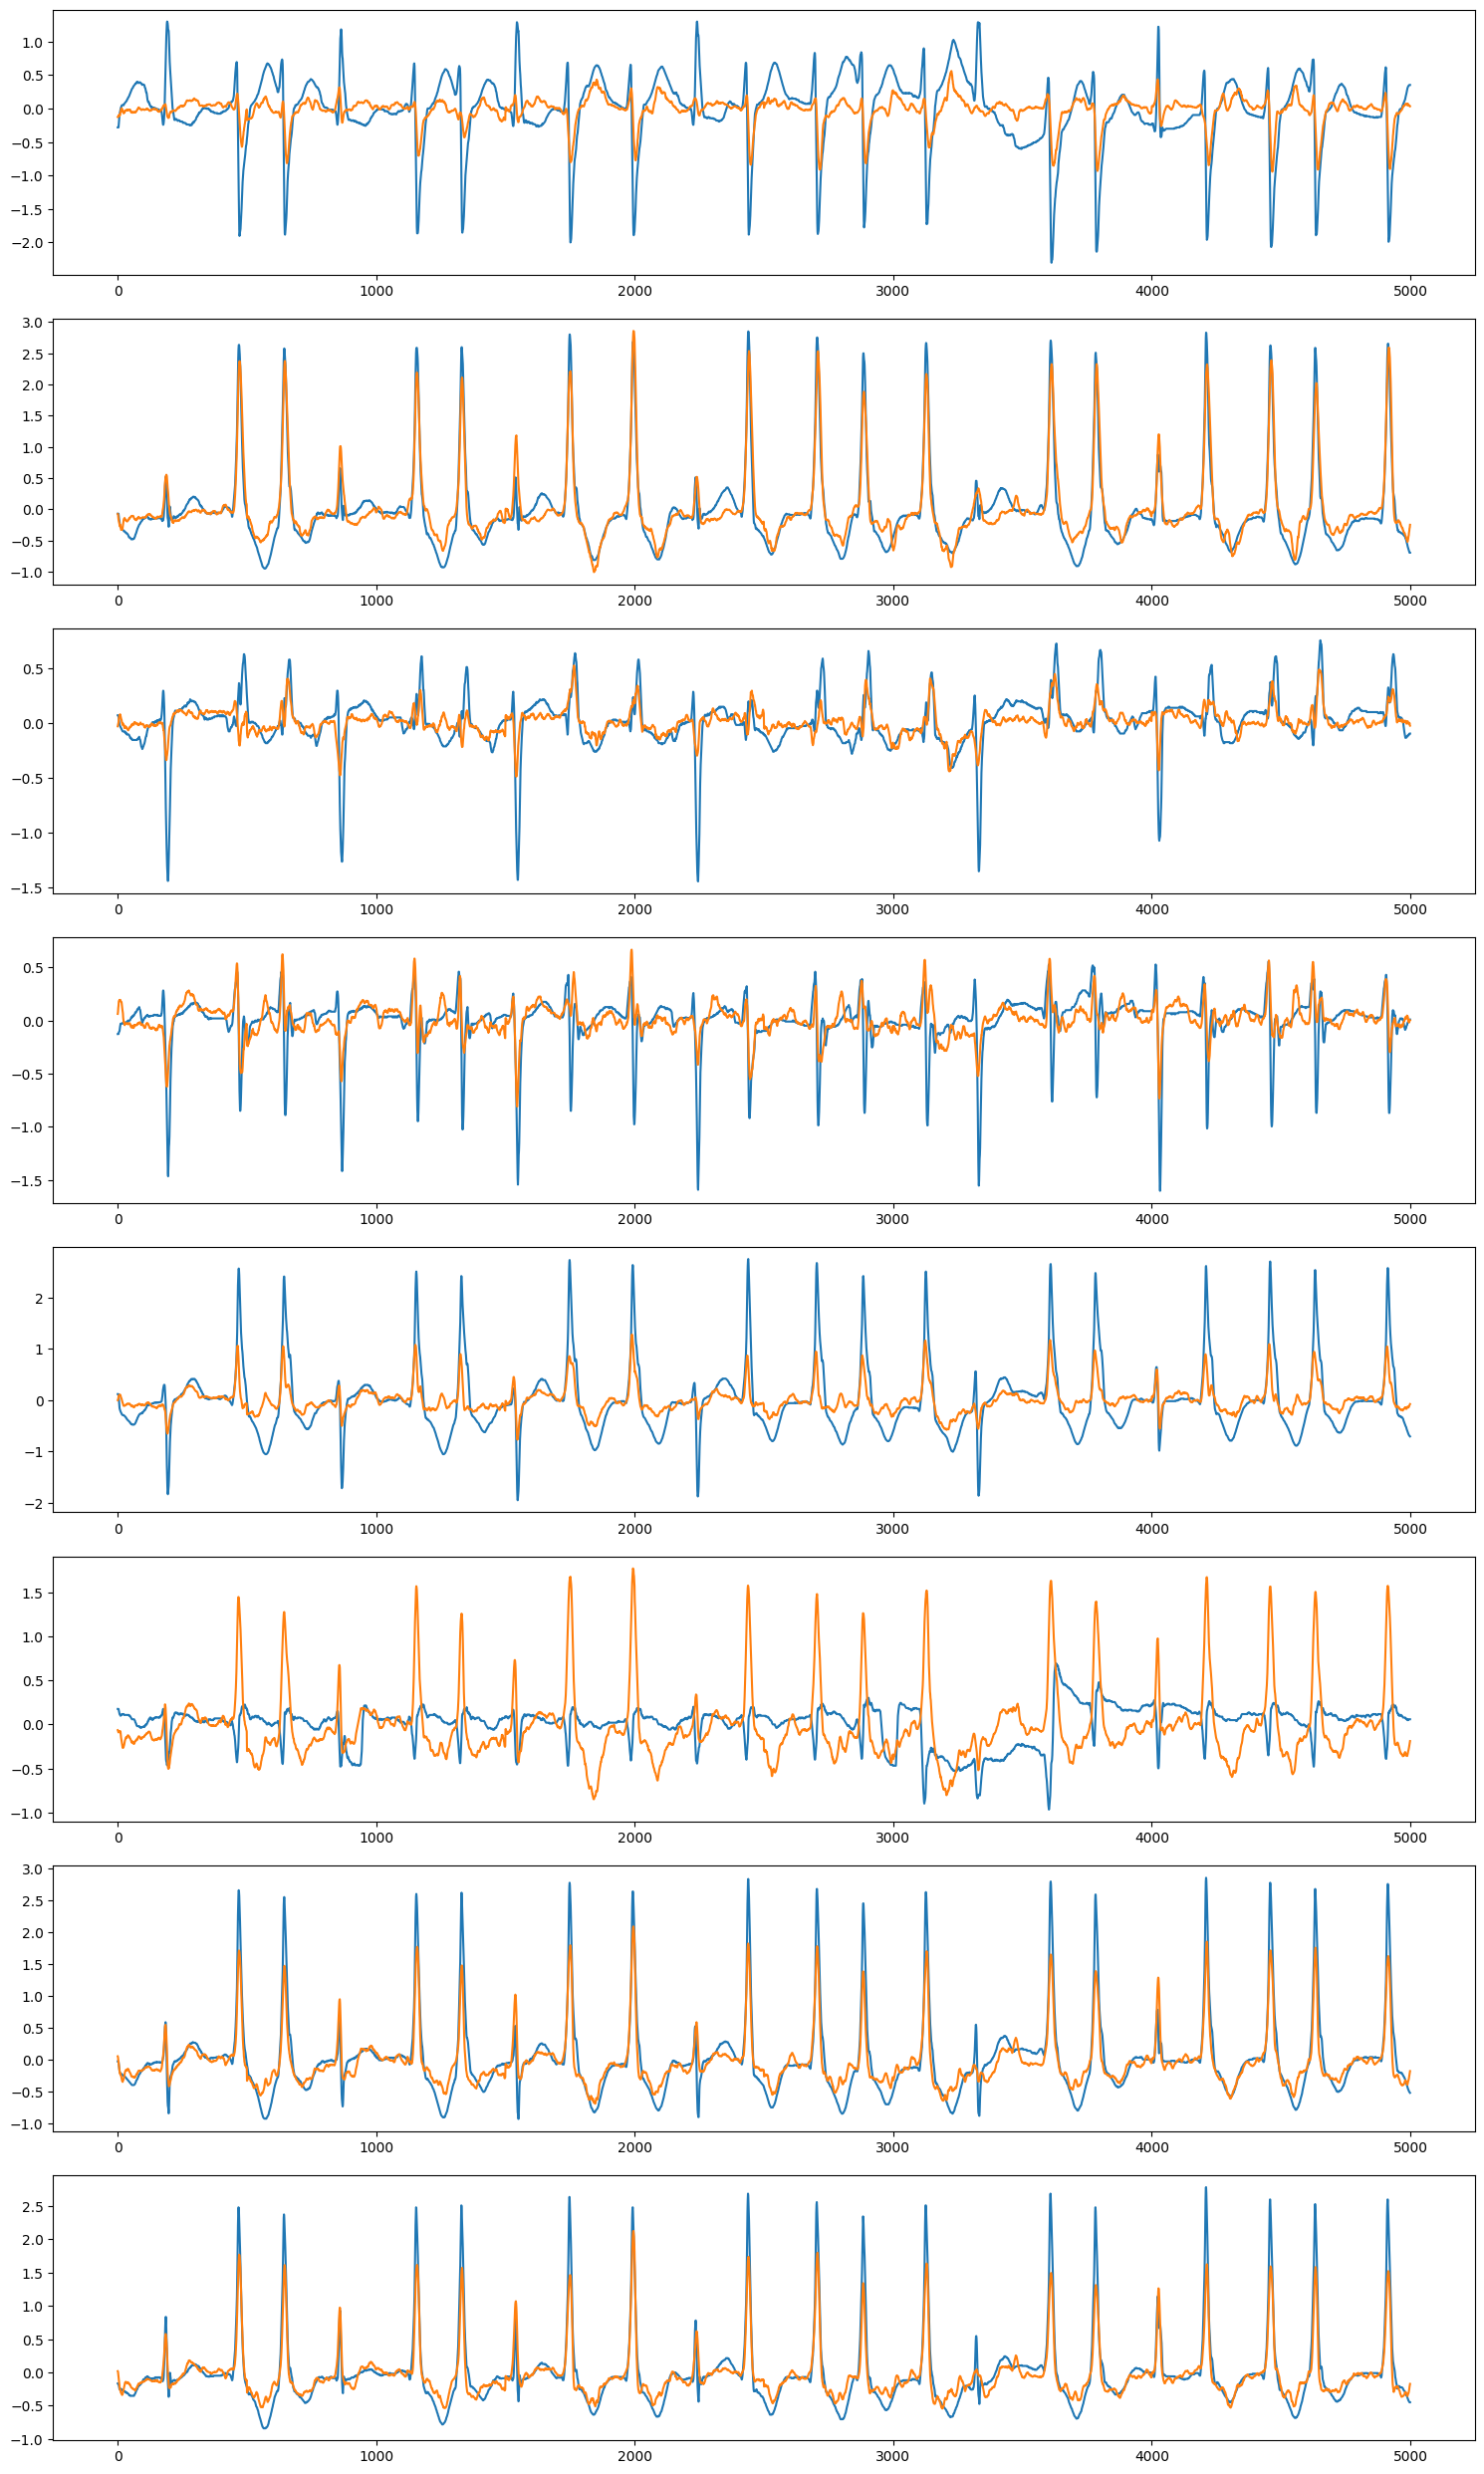
\includegraphics[width=0.93\textwidth]{fp_example.png}
		\caption{Clean example with high reconstruction loss (FP). Blue is the original signal, while orange is the AE reconstruction.}% 
		\label{fig:fp_example}
	\end{figure}

	\item High frequency Gaussian noise is often small in amplitude, resulting in small reconstruction loss, which increases the FNR. \Cref{fig:fn_example} presents an ECG which contains high-frequency noise, but its overall form is approximated well by the AE, resulting in small reconstruction loss. 

	\begin{figure}[htbp]
		\centering
		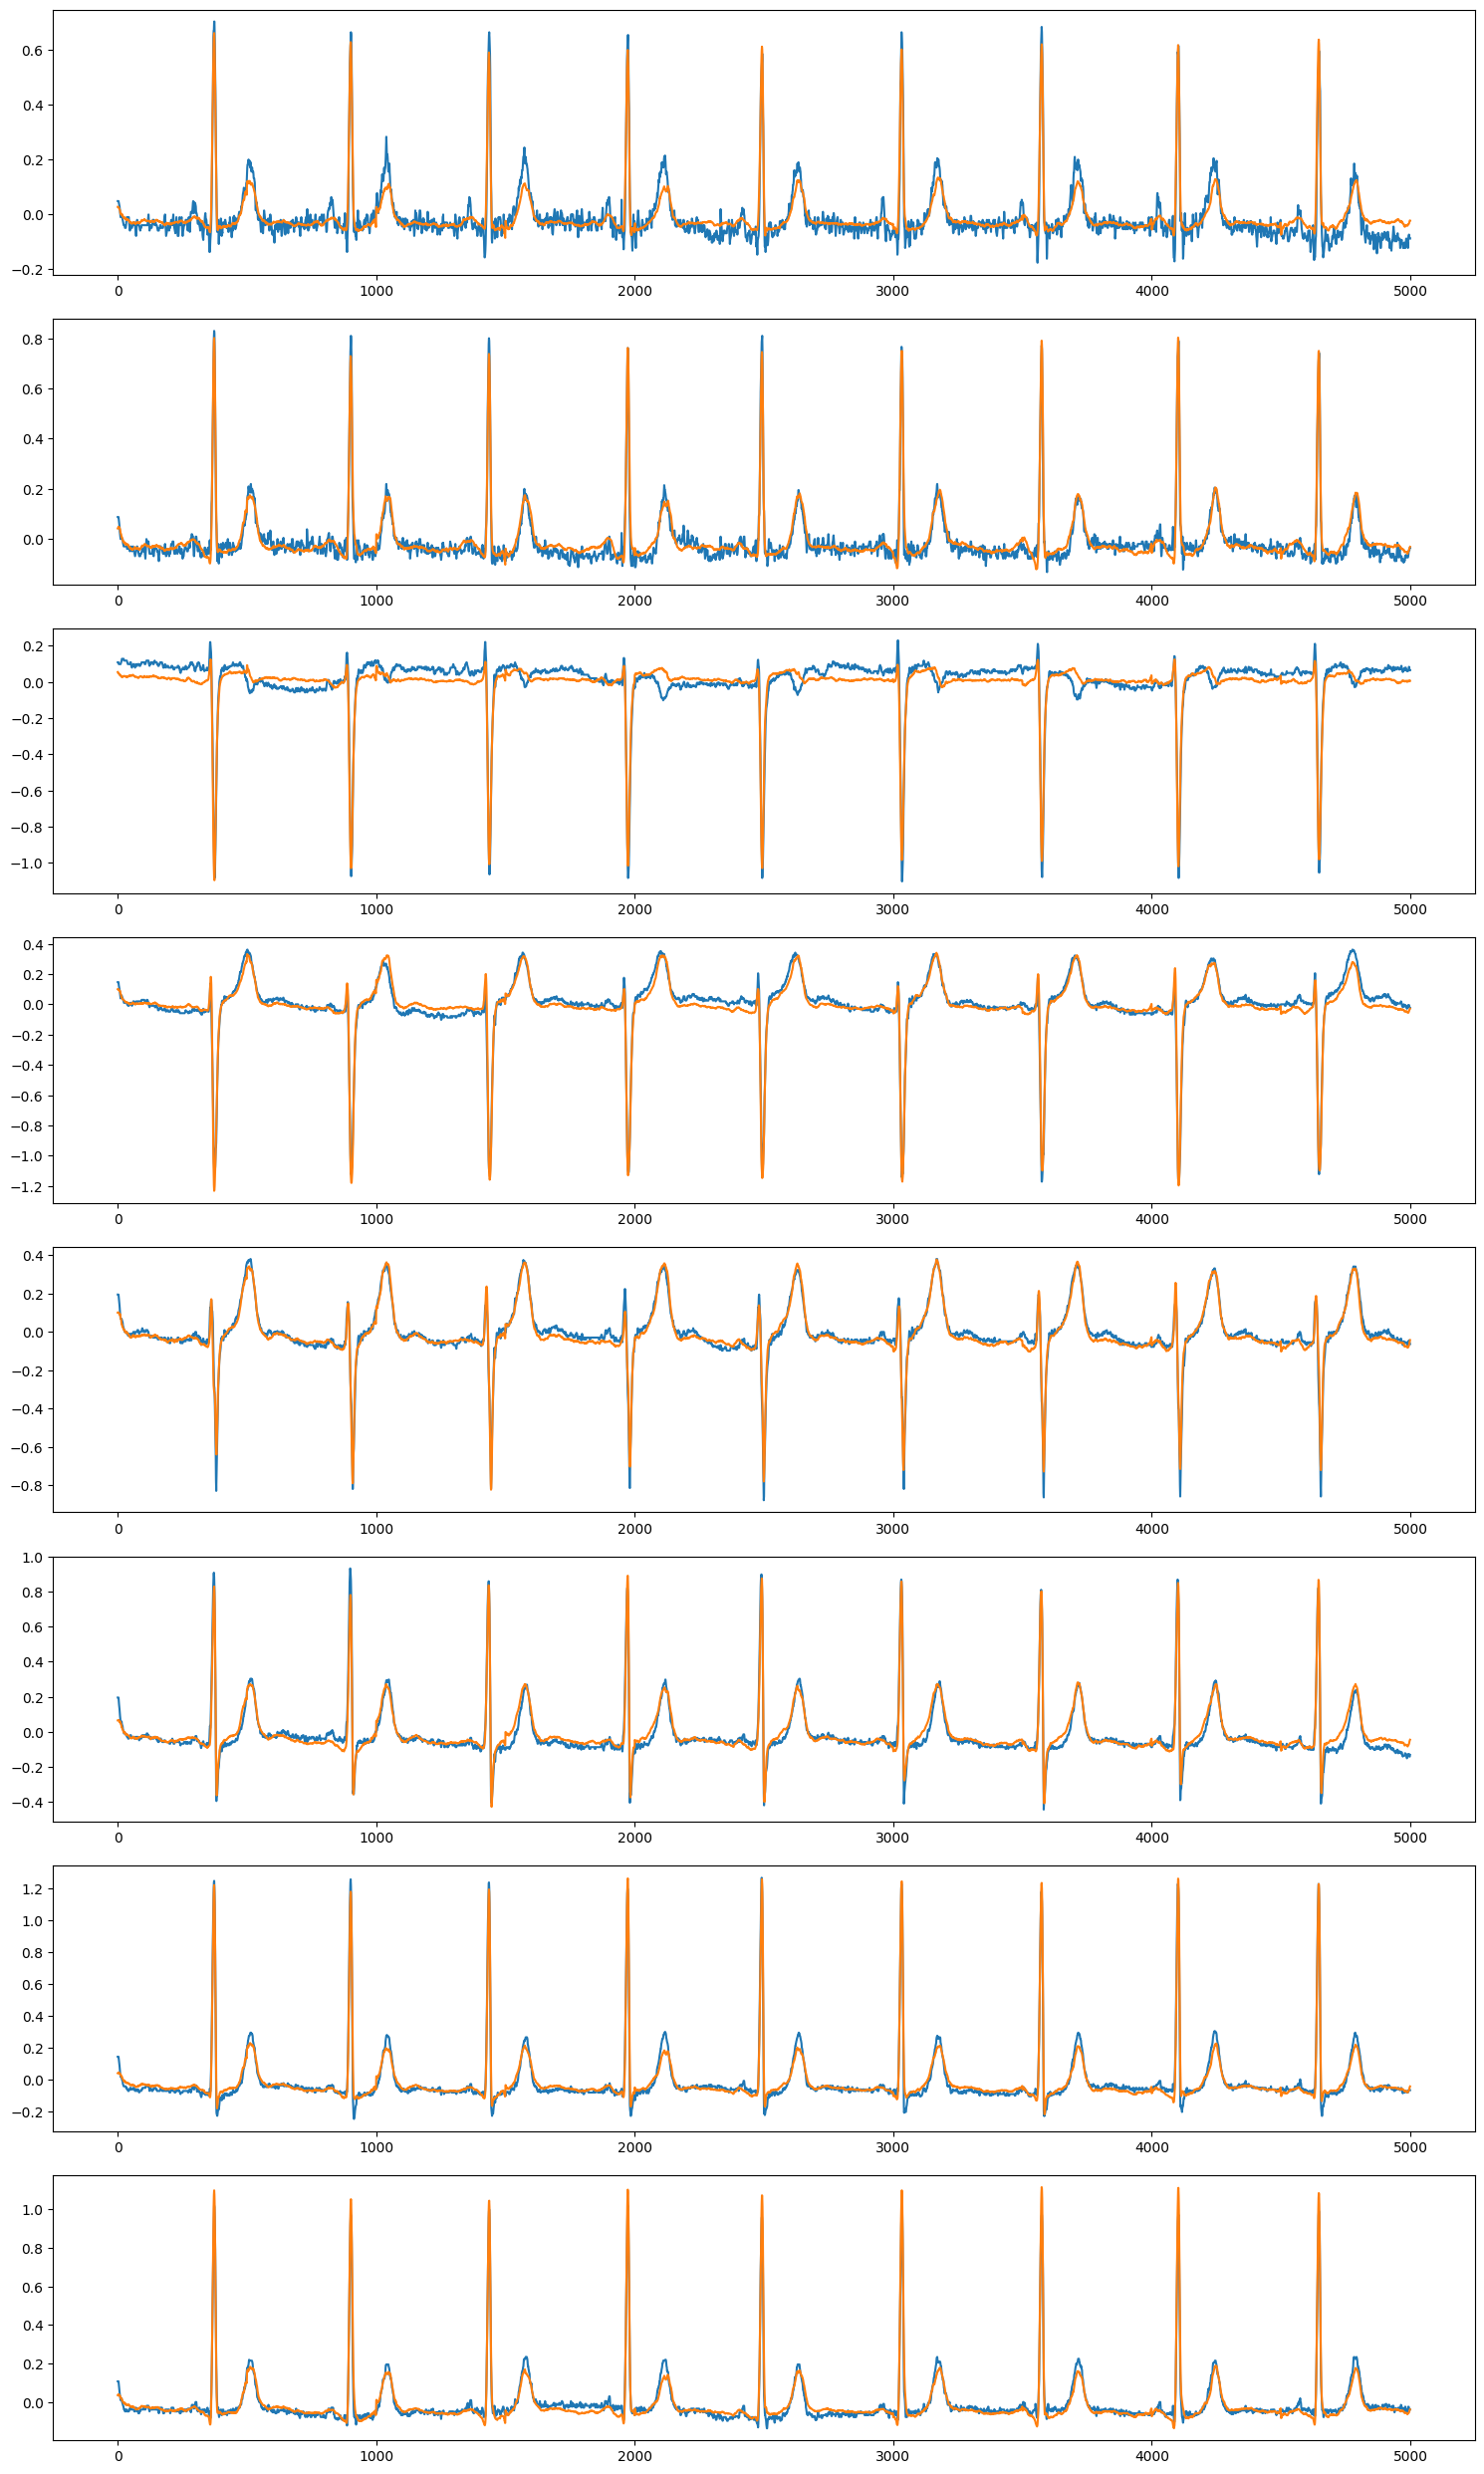
\includegraphics[width=0.93\textwidth]{fn_example.png}
		\caption{Noisy example with low reconstruction loss (FN). Blue is the original signal, while orange is the AE reconstruction.}% 
		\label{fig:fn_example}
	\end{figure}

	\item The scale of the ECG can affect the scale of the loss. In particular:
	      \begin{itemize}
		      \item Noisy ECGs with small amplitudes might also produce reconstructions with small amplitudes, and therefore small reconstruction loss, increasing the FNR.
		      \item Autoencoders tend to produce small neural activations when presented with unfamiliar inputs, whether those are genuinely OOD, or rare conditions that are under-represented in the training data \cite{rethinking}. The former case increases the FNR as explained above, while the latter case increases the FPR.
	      \end{itemize}
\end{itemize}

\paragraph{Dealing with FP.} The following techniques were used to help counter the issue of abnormal rhythms being flagged as FP (\ref{RQ:noise_vs_abnormal}):
\begin{itemize}
	\item \emph{Random augmentations} were introduced to the training set with the aim of better familiarizing the autoencoder with different ECG presentations. Data augmentation techniques are widely used in many domains in order to produce more robust models. However, our options for augmentations are more limited in the noise detection task. Indeed, it is important not to introduce noise to the training data, otherwise we are running into the risk of the model overfitting and producing good reconstructions for noise as well. The study \cite{augmentations} investigates a number of augmentations (albeit for the different task of contrastive representation learning of ECGs). In the end the following augmentations were applied:
	      \begin{itemize}
		      \item \emph{Random shift}: The signals were shifted in the time dimension by a random factor. Mirroring was used to fill in the blank space left behind by the shifting.
		      \item \emph{Baseline drift:} Small amounts of baseline drift were randomly applied on the signal. Large baseline drift may be classified as noise, but small amounts still leave behind an interpretable signal.
		      \item \emph{Permutation:} Following \cite{augmentations}, the ECG are split into $n$ parts of equal size in the time dimension. The parts were then permuted randomly in order to create a new ECG. This technique can actually introduce noise, so it is important to apply it sparingly and to ensure that $n$ is approximately equal to  number of heartbeats expected to be found in the ECG based on its length (e.g.\ $n=10$ in our case, see \cite{augmentations}).
	      \end{itemize}
	\item \emph{Weighted sampling} was used in order to increase the model's familiarity with rare conditions. The weights applied for each sample were determined as follows:
	      \begin{itemize}
		      \item For each sample, its least frequent diagnostic label of interest is determined.
		      \item The sample receives a weight inversely proportional to the frequency of its least frequent label.
		      \item Additionally, when testing on the validation set, the classes that most often appear as FP receive an increased weight.
	      \end{itemize}
\end{itemize}

Other ideas were also attempted in order to deal with the issue of FP, including:
\begin{itemize}
	\item A DiagCl model (see \refsec{sec:diagcl_architecture}) was trained on the diagnostic labels. The weights of the classifier were then frozen. During training of the AE, the reconstruction produce by the AE was input in the trained classifier. A weighted sum of the reconstruction loss and the classifier loss was used for optimisation. The idea here is to force the network to make representations that better capture the unique features of each diagnostic label.
	\item An encoder was pretrained using SimCLR (see \refsec{sec:simclr_architecture}), and then finetuned as a part of the AE system. The idea here is that better weight initialization as well as better encodings in the AE's latent space may lead to better reconstructions overall.
\end{itemize}
These ideas were abandoned however, because they did not seem to result in significant improvements.

\paragraph{Dealing with FN.} Dealing with false negatives is a harder task, since more training leads to better reconstructions, which also applies to noisy ECGs, which then increases the FN rate. One idea is to try and deal with high-frequency noise separately, by examining the frequency components of each signal using a Fourier Transform. In particular, we apply a 4th-order low-pass Butterworth filter \cite{butterworth} with a cutoff frequency at 40 Hz, which should not affect most normal ECGs that are mainly concentrated in the 0.05-35 Hz range \cite{ecgstats}. The Butterworth filter is a standard signal processing tool. In short, it works by multiplying each frequency found in the signal by a certain factor in order to leave the desired frequencies mostly unchanged, while minimising the contribution of unwanted frequencies. \Cref{fig:butterworth_fr} shows the frequency response of the Butterworth filter used in this work; the cutoff frequency (i.e.\ the frequency with voltage gain of $1\big/\sqrt{2} \approx 0.7071$, which is 40 Hz here) is highlighted in red.
\begin{figure}[htbp]
	\centering
	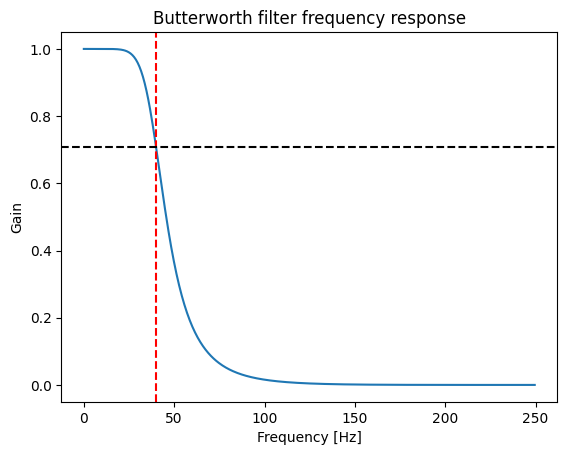
\includegraphics[width=0.6\textwidth]{butterworth.png}
	\caption{Frequency response for 4th-order low-pass Butterworth filter with a cutoff frequency at 40 Hz.}% 
	\label{fig:butterworth_fr}
\end{figure}
We attempt to detect ECGs with high-frequency noise as follows. For each ECG $x$ let $x'$ be the resulting signal after $x$ passes through the filter. We calculate the $L_1$-norm of $x-x'$, i.e.:
\[
	L_1(x, x') = \sum_{c=1}^{8}\sum_{i=1}^{5,000}|x_{c,i} - x'_{c,i}|.
\]
Signals with high $L_1$-norm are considered noisy. Classification happens based on a fixed threshold of 500. This rule filters 17\% of the noisy data while still letting through 98\% of the clean data.

\paragraph{Dealing with scaling.} As explained in \refsec{sec:data_normalisation}, the data is not normalised during training, since the scale of the ECGs has diagnostic meaning, and the noise is scale-dependent. However, scaling can be used upon inference in order to help mitigate the effect of the ECG's scale on the reconstruction loss. Following \cite{rethinking}, instead of the MSE loss we use the following scaled Euclidean distance upon inference:
\[
	L_{2-scaled}(x,y) = \left\|\frac{x}{\|x\|} - \frac{y}{\|x\|}\right\|,
\]
where $x$ is the input and $y$ is the reconstruction. Note that since any input $x$ that contain all 0s can easily be detected by our rule based system, in practice it the above distance should always be defined.

\paragraph{Training.} We report on the training of the most successful model with respect to the noise detection task. The AE was trained over 30 epochs on Clean split A using the AdamW optimiser \cite{adamw} and the OneCycle learning rate scheduler \cite{onecyclelr}, which starts the learning rate from a small value, increases it over 3 epochs to its max value of $10^{-3}$, and then gradually decreases to almost 0 over the rest of the epochs via a cosine annealing strategy. The model with the smallest validation loss, achieved at epoch 28, is kept for further testing. \Cref{fig:ae_metrics} shows the training and validation losses per epoch.

\subsubsection{Results}

Our most successful model is rather large, at 51.9 million parameters. Multiple attempts were made to reproduce its results with smaller models using different training hyper-parameters; however, these attempts were largely unsuccessful.

\paragraph{Clean split A.} Training using random augmentations and weighted sampling improved the performance of the model to a ROC-AUC of 0.684 (95\% CI: [0.679, 0.690]). \Cref{fig:label_dist} shows the label distribution in the FP compared to the distribution of the clean samples for the same threshold. We observe that many of the abnormal classes are excessively flagged as FP, which indicates a bias in the model, since FP are also clean by definition. The distribution remains biased after applying random augmentations and weighted sampling, however the differences are less pronounced in some abnormal labels (see e.g.\ labels \emph{class\_abnorm}, \emph{rhythm\_st}, \emph{conduction\_rbtb}, etc.).
\begin{figure}[htbp]
	\makebox[\linewidth][c]{
		\begin{subfigure}[b]{1.2\textwidth}
			\centering
			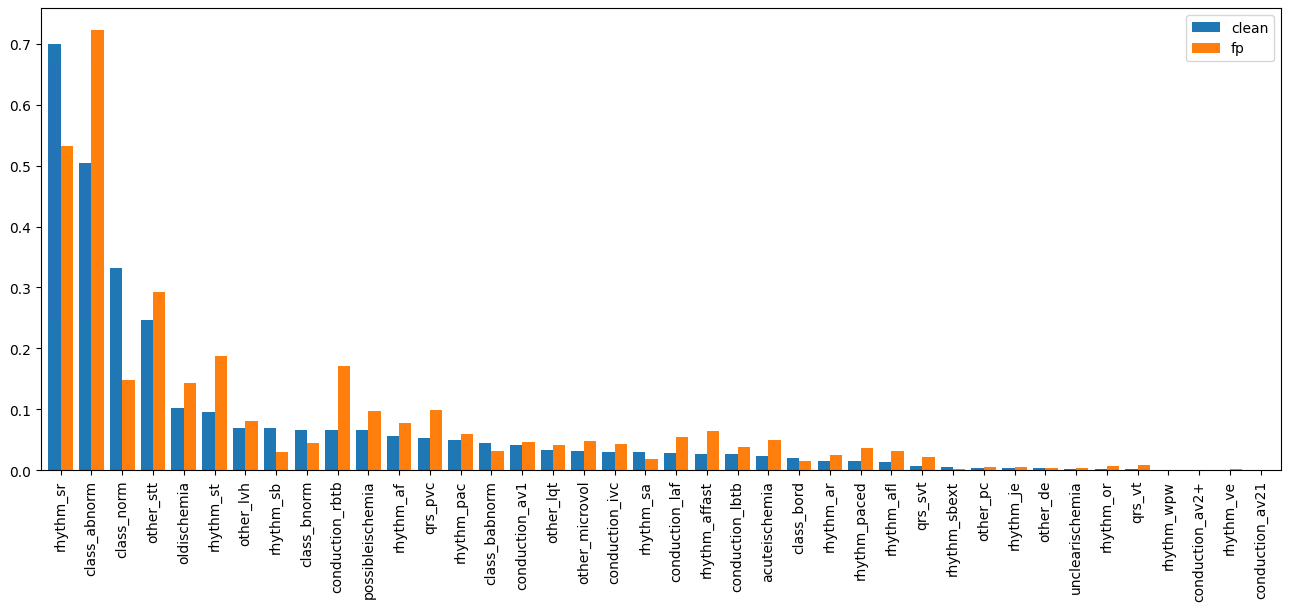
\includegraphics[width=\textwidth]{label_dist_fp_clean_non_finetuned.png}
			\caption{Label distribution in false positives before weighting.}% 
			\label{fig:beforeweight}
		\end{subfigure}
	}
	\vskip\baselineskip
	\makebox[\linewidth][c]{
		\begin{subfigure}[b]{1.2\textwidth}
			\centering
			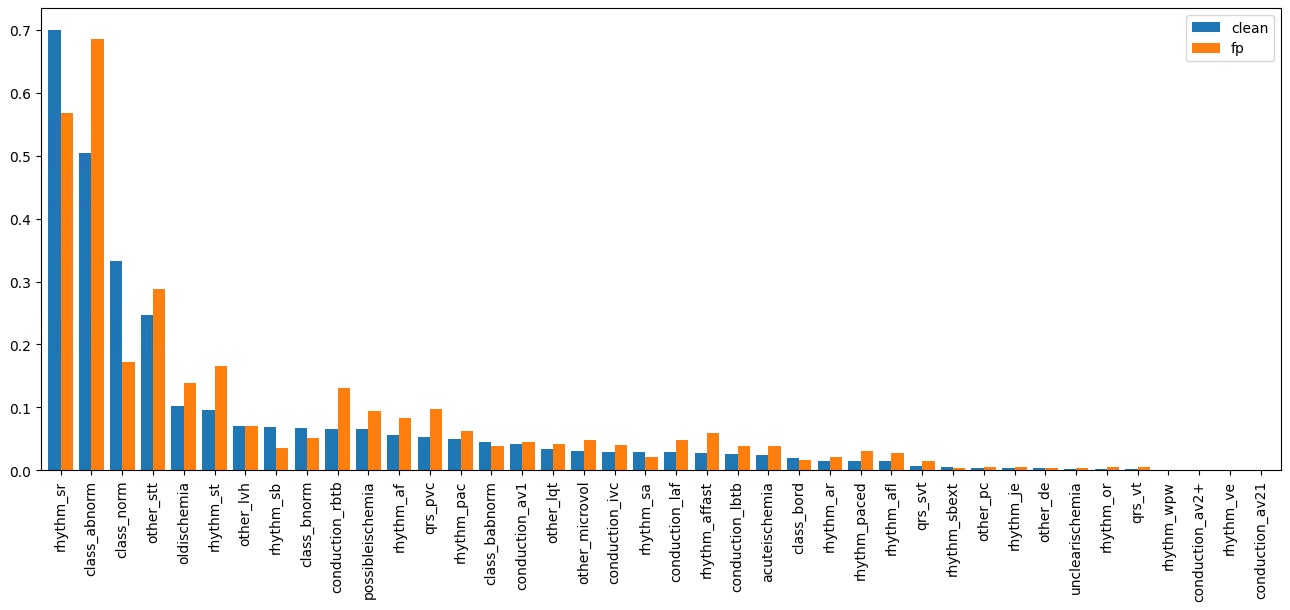
\includegraphics[width=\textwidth]{label_dist_fp_clean.png}
			\caption{Label distribution in false positives after weighting.}% 
			\label{fig:afterweights}
		\end{subfigure}
	}
	\caption{Diagnostic label distribution in FP compared with clean samples before and after augmentations and weighted sampling.}
	\label{fig:label_dist}
\end{figure}

Scaling further increases the ROC-AUC to 0.732 (95\% CI: [0.727, 0.737]). Testing on the noisy data after they are filtered with the Butterworth filter however decreases the ROC-AUC to 0.717 (95\% CI: [0.711, 0.723]).

We choose a classification threshold of 20 on the reconstruction losses empirically based on the best model performance (scaling, no Butterworth filter). With this threshold we get overall accuracy of 0.70. The ROC curve, the scaled confusion matrix and the classification report are found in \Cref{fig:ae_clean_a_roc}, \Cref{fig:ae_clean_a_cm} and \Cref{tab:ae_clean_a_cr} respectively.

\paragraph{Clean split B.} The model achieves slightly better results when tested on Clean split B, with ROC-AUC of 0.698 (95\% CI: [0.692, 0.703]) without scaling and 0.740 (95\% CI: [0.735, 0.745]) with scaling. When the data is reduced by the Butterworth filter the ROC-AUC decreases again to 0.724 (95\% CI: [0.719, 0.730]). Using the same threshold as in split A we obtain accuracy of 0.72. The ROC curve, the scaled confusion matrix and the classification report are found in \Cref{fig:ae_clean_b_roc}, \Cref{fig:ae_clean_b_cm} and \Cref{tab:ae_clean_b_cr} respectively.

\paragraph{Expert-annotated data.} The model achieves ROC-AUC of 0.723 (95\% CI: [0.557, 0.863]) without scaling and 0.760 (95\% CI: [0.611, 0.891]) when scaling is applied. Thresholding as in Clean split A, we get an accuracy of 0.71. \Cref{fig:ae_segm_roc}, \Cref{fig:ae_segm_cm} and \Cref{tab:ae_segm_cr} present the ROC curve, the scaled confusion matrix and the classification report for this classifier on the expert-annotated data.

\paragraph{PhysioNet 2011 data.} The model achieves ROC-AUC of 0.970 (95\% CI: [0.940, 0.991]) without scaling and 0.968 (95\% CI: [0.940, 0.989]) with scaling. When thresholding with the same value as before, we get an accuracy of 0.79. We present the ROC curve, the scaled confusion matrix and the classification report in \Cref{fig:ae_clean_b_roc}, \Cref{fig:ae_clean_b_cm} and \Cref{tab:ae_clean_b_cr} respectively.


\subsection{Feature space clustering}

We now move on to the experimentation process for the feature space clustering method, which is explained in \refsec{sec:fs_method}.

\subsubsection{Experiments}

For the feature space clustering experiments we choose a feature space of 128 dimensions. As mentioned, the three architectures that were used for the feature space clustering experiments were AE, DiagCl and SimCLR. Once each architecture was trained for its particular task, the double residual encoder part of each was extracted in order to obtain a feature extractor
\[
	F: \R^{8\times5000} \to \R^{128}.
\]
For the AE training process refer to \refsec{sec:ae_exp}. For the DiagCl training process refer to \refsec{sec:uncertainty_exp}. In this section we only discuss the SimCLR training process.

\paragraph{SimCLR Loss.} As mentioned in \refsec{sec:fs_method}, the loss used for the training of SimCLR is the InfoNCE loss, which is described in detail in \cite{infonce}.

\paragraph{SimCLR training.} We train the SimCLR architecture on Clean split A over 30 epochs using the AdamW optimiser and the OneCycle learning rate scheduler, with maximum learning rate of $10^{-4}$. The training and validation losses over the training epochs are shown in \Cref{fig:simclr_metrics}.

\paragraph{In-distribution embeddings.} The in-distribution embeddings are obtained via the 294,046 ECGs in the training set of Clean split A. The embeddings are then clustered using a GMM. The model was tested using 1-4 clusters. We also tried reducing the number of dimensions using PCA while keeping 99\% of the data's variance, and clustering on the reduced data.

\subsubsection{Results}

\paragraph{Clean split A, Clean split B, expert-annotated set.} This method did not seem to achieve any useful separation between the two classes for any of the UMCU splits, consistently failing to reach ROC-AUC above 0.6 regardless of the number of clusters used for the GMM or whether the embeddings were reduced or not. \Cref{tab:roc-auc_feature_umcu} shows the best ROC-AUC scores for each feature extractor (all of which were achieved for a single GMM cluster of the data). We do not report on any further classification metrics for these splits, as they are not of interest.

\begin{table}[htbp]
	\centering
	\begin{tabular}{r|c|c|c}
		                          & \textbf{AE} & \textbf{DiagCl} & \textbf{SimCLR} \\ \midrule
		\textbf{Clean split A}    & 0.512       & 0.514           & 0.523           \\
		\textbf{Clean split B}    & 0.526       & 0.517           & 0.531           \\
		\textbf{Expert-annotated} & 0.552       & 0.554           & 0.555
	\end{tabular}
	\caption{ROC-AUC of each feature space extractor for each UMCU split.}
	\label{tab:roc-auc_feature_umcu}
\end{table}

\Cref{fig:feature_clean_a_dist} compares the distribution of the Mahalanobis distances of the clean and the OOD data of the Clean split A test set from the training-data distribution, as calculated by a single cluster GMM. Ideally we would expect some separation between the two, with the OOD distances having generally higher values. However, the distributions seem almost identical. \Cref{fig:feature_clean_a_pca} shows 2-D PCA plots of the embeddings obtained from the training set, as well as the clean and the noisy parts of the Clean split A test set. Once again, we observe no separation between their distribution in space.

\begin{figure}[htbp]
	\makebox[\linewidth][c]{
		\begin{minipage}{0.6\textwidth}
			\centering
			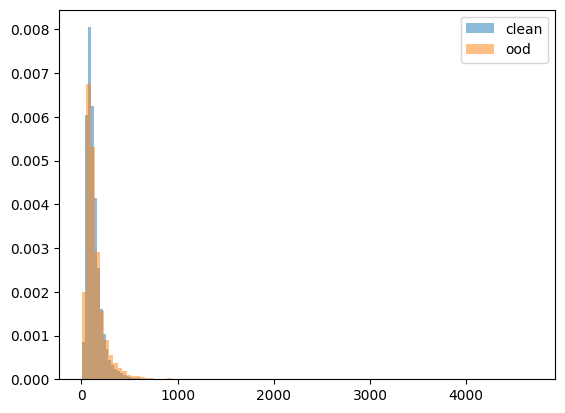
\includegraphics[width=\textwidth]{feature_clean_a_dist.png}
			\caption{Mahalanobis distance distribution for AE on Clean split A.}% 
			\label{fig:feature_clean_a_dist}
		\end{minipage}
		\hspace{0.1cm}
		\begin{minipage}{0.6\textwidth}
			\centering
			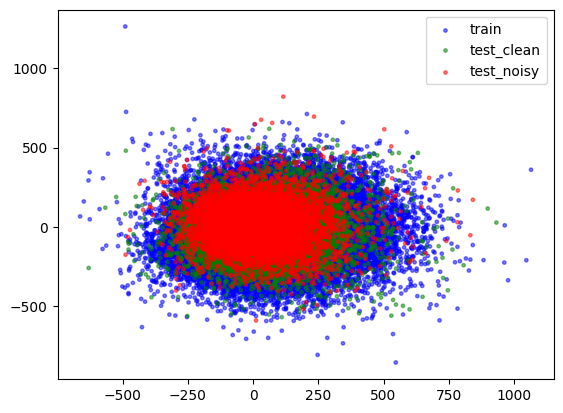
\includegraphics[width=\textwidth]{feature_clean_a_pca.png}
			\caption{PCA on features extracted from AE on Clean split A.}% 
			\label{fig:feature_clean_a_pca}
		\end{minipage}
	}
\end{figure}

\paragraph{PhysioNet 2011 data.} The algorithm had surprisingly strong performance on the PhysioNet 2011 data:
\begin{itemize}
	\item AE achieved a max ROC-AUC of 0.931 (95\% CI: [0.896, 0.960]).
	\item DiagCl achieved a max ROC-AUC of 0.840 (95\% CI: [0.725, 0.935]).
	\item SimCLR achieved a max ROC-AUC of 0.933 (95\% CI: [0.865, 0.972]).
\end{itemize}
The above scores were obtained for a single GMM cluster after PCA was applied. In particular for SimCLR, by keeping 99\% of the data's variance we go down from 128 to 6-dimensions. The ROC curve for this classifier can be seen in \Cref{fig:feature_phynet_roc}. By comparing the Mahalanobis distances of the test samples with the CDF of the chi-squared distribution with 6 degrees of freedom, and rejecting a sample $x$ as noisy if
\[
	P(X \leq M(x, D_{train})) = 0.99 \iff P(X \geq M(x, D_{train})) = 0.01
\]
(where $X$ denotes a random variable that follows the chi-squared distribution with 6 degrees of freedom), we get a classifier that achieves accuracy of 0.82. The confusion matrix and classification report for this classifier show strong performance on the noise detection task, and can be found in \Cref{fig:feature_phynet_cm} and \Cref{tab:feature_phynet_cr} respectively.


\subsection{Uncertainty based methods}

Finally, building upon \refsec{sec:un_method}, we discuss our experiments with uncertainty as a measure of noise.

\subsubsection{Experiments}
\label{sec:uncertainty_exp}

For this method we mainly use the DiagCl architecture (see \refsec{sec:diagcl_architecture}).

\paragraph{Loss.} As explained in the corresponding section, the DiagCl model is simply an encoder with 5 independent classification heads, 4 of which correspond to multi-class problems, while the other is multi-label. As a result, the DiagCl model is optimised with respect to a weighted average of 4 Cross Entropy (CE) losses and 1 Binary Cross Entropy (BCE) Loss.

\paragraph{Training.} The model is trained on Clean split B over 30 epochs using the AdamW optimizer and the ReduceLROnPlateau learning rate scheduler, starting with a learning rate of $10^{-4}$. Random augmentations as well as weighted sampling are used during the traing process. Weight initialisation by a pre-trained SimCLR network was also attempted, without leading to huge improvements. The above process is repeated 5 times, using different random weight initializations each time. The training metrics can be found in \Cref{fig:ens_metrics}.

\paragraph{Uncertainty estimation.} The dropout layers of each network's classification heads remain active upon inference. Given an input $x$, 4 different predictions are made by each network using randomly generated dropout masks. As a result, for each unique input $x$ we get $5\times 4 = 20$ independent diagnostic label predictions. The mean of these predictions can be used for inference, while their variance can be used as a measure of epistemic uncertainty, effectively combining the ensemble and Monte Carlo methods for uncertainty estimation.

\paragraph{Ensemble's predictive capabilities.} The ensemble shows good performance overall on the task at which it was trained for, although it does struggle with a few under-represented classes. Detailed classification metrics can be found in \Cref{fig:diagcl_rhythm_cm,fig:diagcl_avc_cm,fig:diagcl_vc_cm,fig:diagcl_ischemia_cm,tab:diag_other_roc-auc}.


\subsubsection{Results} We aim to use the uncertainty estimation as a measure of noise (\ref{RQ:uncertainty}), with our hypothesis being that high uncertainty may indicate an OOD ECG. When testing on any of the three test sets however, we observe the opposite effect, obtaining ROC-AUC less than 0.5 on every set. Plotting the uncertainty estimations for the clean and the noisy data of the test set of Clean split B, we see that it is indeed common for the classifier to exhibit higher uncertainty in the clean data rather than the noisy data. Counterintuitively, this effect is even more pronounced with the data that is in Clean split A but not in Clean split B, i.e.\ those that are excluded purely because of their diagnostic labels; the classifier seems to exhibit even less uncertainty on this data (referred to as ``mislabelled'' in \Cref{fig:uncertainty_umcu}).

\begin{figure}[htbp]
	\centering
	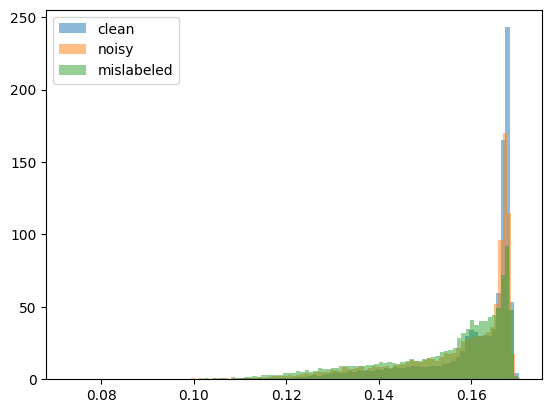
\includegraphics[width=0.7\textwidth]{uncertainty_umcu.png}
	\caption{Uncertainty estimations for the Clean split B test data, as well as the ``mislabelled'' data.}
	\label{fig:uncertainty_umcu}
\end{figure}

A similar effect is observed in the corresponding plots for the expert-annotated set and the PhysioNet 2011 data (\Cref{fig:uncertainty_segm} and \Cref{fig:uncertainty_phynet} respectively).

\begin{figure}[htbp]
	\centering
	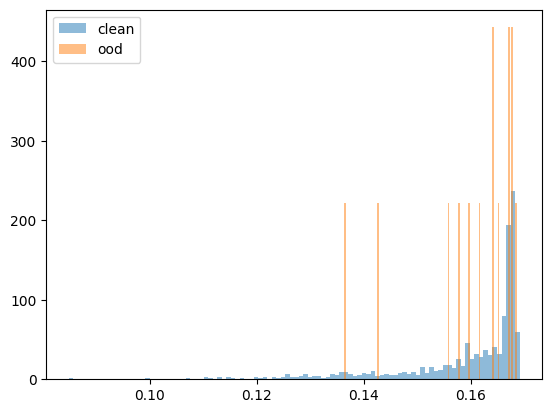
\includegraphics[width=0.7\textwidth]{uncertainty_segm.png}
	\caption{Uncertainty estimations for the expert-annotated data.}
	\label{fig:uncertainty_segm}
\end{figure}

\begin{figure}[htbp]
	\centering
	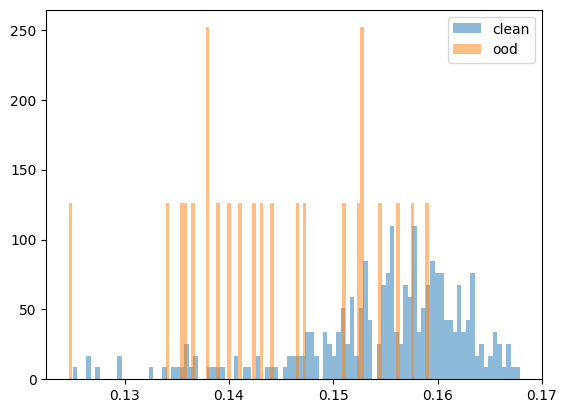
\includegraphics[width=0.7\textwidth]{uncertainty_phynet.png}
	\caption{Uncertainty estimations for the PhysioNet 2011 data.}
	\label{fig:uncertainty_phynet}
\end{figure}


\subsection{Summary of best ROC-AUC scores}

\Cref{tab:best-roc-auc} summarises the maximum ROC-AUC scores that each method achieved on each dataset that it was tested on.

\begin{table}[htbp]
	\begin{tabular}{r|c|c|c|c}
		                       & \textbf{Binary class.} & \textbf{Reconstruction} & \textbf{Feature space} & \textbf{Uncertainty} \\ \midrule
		\textbf{Binary class.} & 0.907                  & \emph{n/a}              & \emph{n/a}             & \emph{n/a}           \\
		\textbf{Clean split A} & \emph{n/a}             & 0.732                   & 0.523                  & \emph{n/a}           \\
		\textbf{Clean split B} & \emph{n/a}             & 0.740                   & 0.531                  & $< 0.5$              \\
		\textbf{Expert-ann.}   & \textbf{0.978}         & 0.760                   & 0.555                  & $< 0.5$              \\
		\textbf{PhysioNet}     & 0.909                  & \textbf{0.970}          & \textbf{0.933}         & $< 0.5$
	\end{tabular}
	\caption{Best ROC-AUC scores achieved by each method on each dataset.}
	\label{tab:best-roc-auc}
\end{table}


\section{Discussion}

We now discuss our results in relation to the research questions as defined in \refsec{sec:research_questions}.

\paragraph{\ref{RQ:OOD_detection}.} Our experiments show that for ECG noise detection, binary classification seems to be by far the preferred method. While supervised learning often provides the best results when labelled data is available, it also has its drawbacks:
\begin{itemize}
	\item Labelled data is not always available, and creating a sufficiently large labelled dataset from the beginning requires expert knowledge and significant time investment. Moreover, the network's performance relies significantly on the label quality (see \refsec{sec:limitations}).
	\item A classifier that has been trained on a single labelled dataset often performs worse for the same task on different datasets. 
	\item The network's decisions are generally hard to explain.
\end{itemize}

The reconstruction methods show some promise on the noise detection task, although they do not reach the same performance as the binary classifier on the UMCU data. Regardless, the AE can be quite useful in a noise detecting pipeline. For a start, its decisions are easy to interpret, as one can visually inspect the reconstructions. Moreover, not all of the FP generated by this method are necessarily FP, as they may also be mislabelled data. \Cref{fig:fp_mislabelled} shows one such example, and during error analysis many more were discovered. On the other hand, as shown by the FN examples in which the AE produced excellent reconstructions without the high-frequency noise, the AE can also be used for noise removal instead of noise detection.

\begin{figure}[htbp]
	\centering
	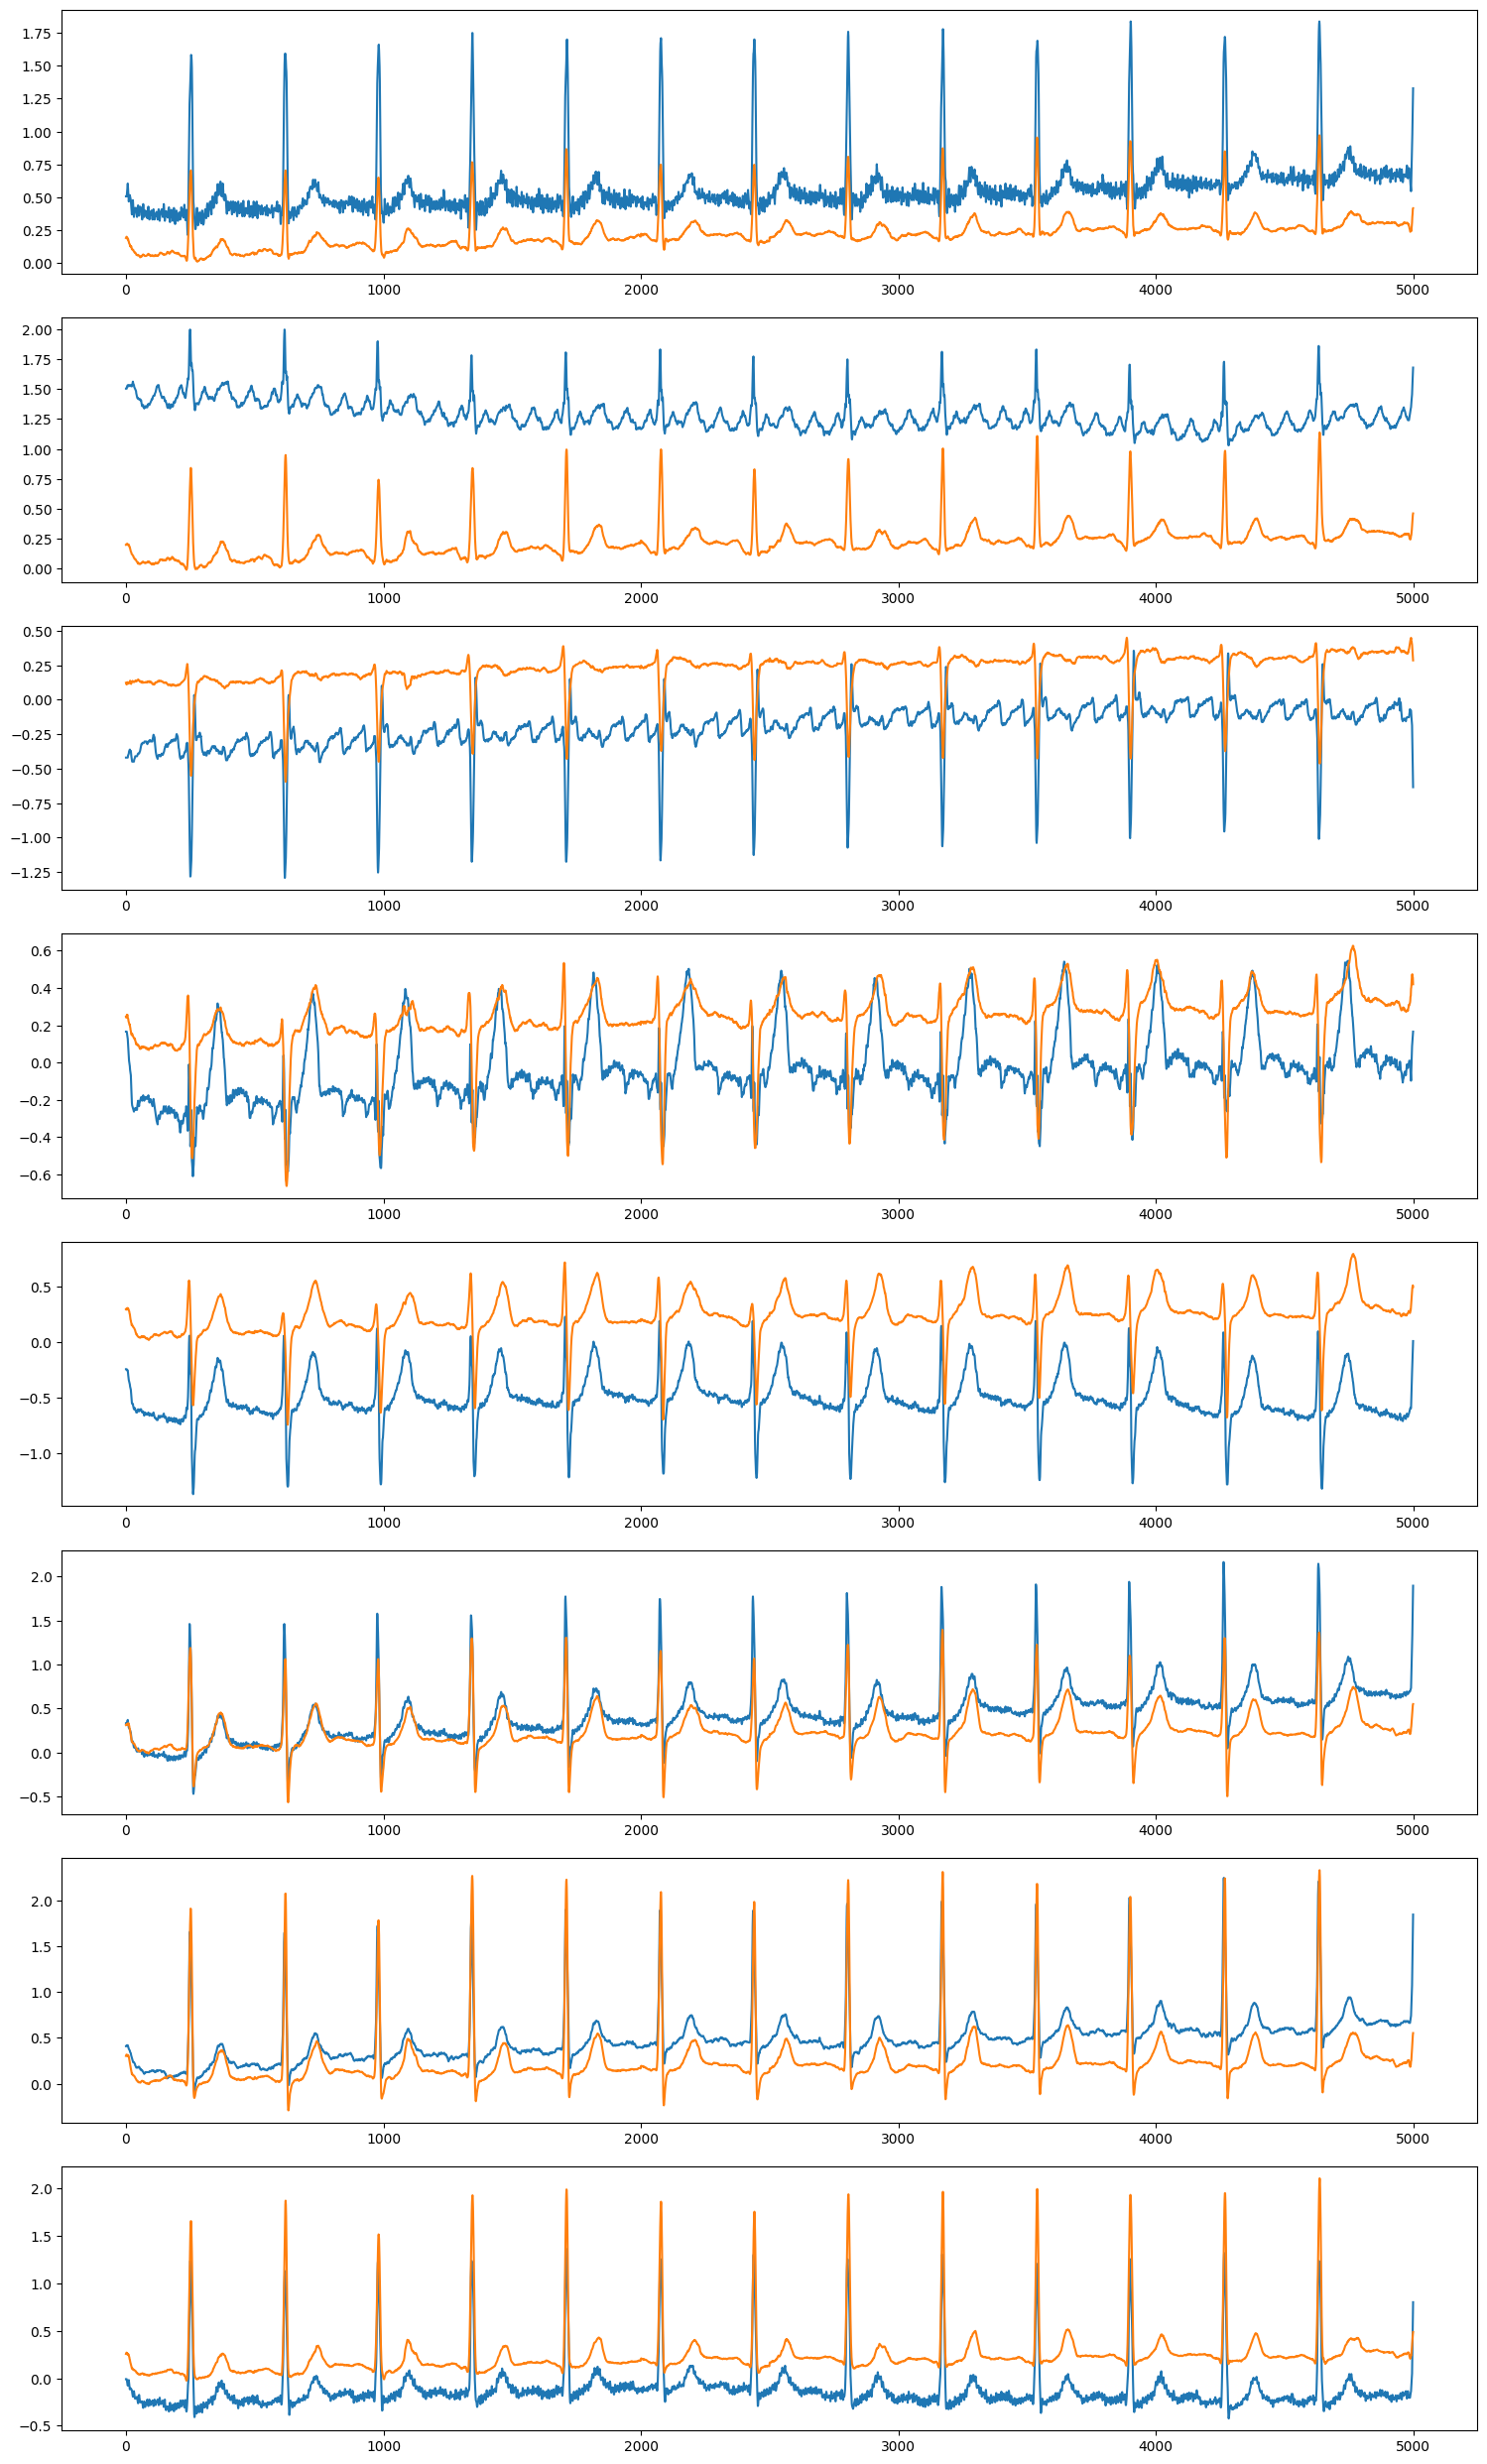
\includegraphics[width=0.93\textwidth]{fp_mislabelled.png}
	\caption{Mislabelled FP sample with high reconstruction loss.}% 
	\label{fig:fp_mislabelled}
\end{figure}

The feature space methods did not produce good results for the noise detection task. While SimCLR is one of the easiest contrastive learning techniques in terms of implementation, it is probably not suitable for this task, as it is trained to produce similar embeddings for similar signals. It is therefore likely that a normal ECG will have a closer embedding to a noisy version of itself rather than to an ECG with severe pathology. Thus, the method is probably more suited for diagnostic anomaly detection.

\paragraph{\ref{RQ:noise_vs_abnormal}.} The two main techniques that were found to be useful for the AE method in particular were the introduction of augmentations and weighted sampling during training. These techniques were also used during the training of the other methods, and improved the results empirically. Other ideas that were attempted, as mentioned in \refsec{sec:ae_exp}, were less successful. More sophisticated methods may be required to achieve better results on this topic.

\paragraph{\ref{RQ:uncertainty}.} So far in our experiments, uncertainty has shown to be unsuccessful in terms of predicting the noise level or the uninterpretability of an ECG. However, our experimentation on this topic is not broad enough to give a conclusive answer.  


\subsection{Limitations}
\label{sec:limitations}

While this study aims to cover a broad selection of techniques, it comes with certain limitations.

\paragraph{Unknown quality of available labels.} Noise generally appears to an extent in almost every ECG signal, so it is often complicated even for an expert to judge the level and type of noise required for an ECG to be considered unsuitable for diagnostic purposes. Moreover, it might be the case that even if some leads (or part of leads) of the ECG are very noisy, those that are left are still sufficient for a diagnosis, at which point it is up to the expert's judgement whether they would label the ECG as noisy or not.

\paragraph{Restriction to 8-lead ECGs.} This work focuses exclusively on classifying 8-lead ECGs as clean or noisy. However, strong arguments can be made for the case of detecting noise in specific leads, or specific parts of each lead instead:
\begin{itemize}
	\item Many, but not all machines produce 8+ lead ECGs. Machines with fewer leads are sometimes used in ambulances or during routine check-ups.
	\item Even if one or more of the leads is noisy, the ECG might still be diagnostically interpretable.
	\item An algorithm trained to recognise noise within a lead might have better performance, since its predictions are not influenced by the other leads.
\end{itemize}
The labels given to the original UMCU dataset however do not specify the location of the noise, as such detailed labelling is significantly more time consuming. While the expert-annotated segmentation dataset was eventually available during the internship, this dataset is much smaller, and by that time the main algorithms and pipelines used in this work had already been developed.


\section{Future Work}

Based on our experimentation and results, we can suggest relevant research directions such as the following.
\begin{itemize}
	\item Regarding \ref{RQ:OOD_detection}, experiments with different number of leads, or including segmentation information may improve the performance of the noise-detection algorithms.
	\item More experimentation is needed with respect to \ref{RQ:noise_vs_abnormal}. The development of dedicated methods to tackle this topic specifically might lead to better results.
	\item Regarding \ref{RQ:uncertainty}, the role of uncertainty, how it relates to ECGs that are hard to interpret, and how it influences the predictions of an automated diagnostic system is a very interesting and potentially rich research topic.
	\item While noise detection itself is important, the task may be modified to better suit the needs of an automated diagnostic system. For example, it might be the case that an ECG with minor or localised noise may still be interpetable by an automated system. Noise removal techniques may also be employed. Whether the exclusion of ECGs that are flagged by an OOD detector leads to more accurate predictions for an automated system is also something that should be tested.
	\item Apart from off-line noise detection, an interesting topic is whether the signal can be detected as noisy at the time of acquisition, using time-series anomaly detection techniques.
\end{itemize}




\clearpage
\printbibliography

\clearpage
\section{Appendix}
\label{sec:appendix}

\vspace{4cm}
\begin{figure}[H]
	\centering
	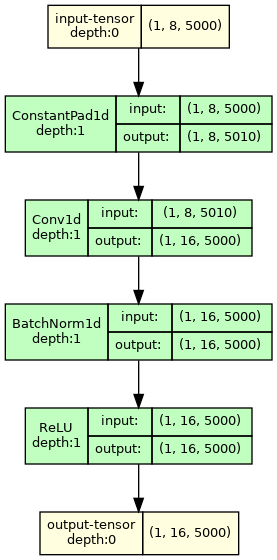
\includegraphics[width=0.4\textwidth]{ConvBlock.gv.png}
	\caption{ConvBlock architecture.}% 
	\label{fig:convblock_architecture}
\end{figure}

\begin{figure}[p]
	\centering
	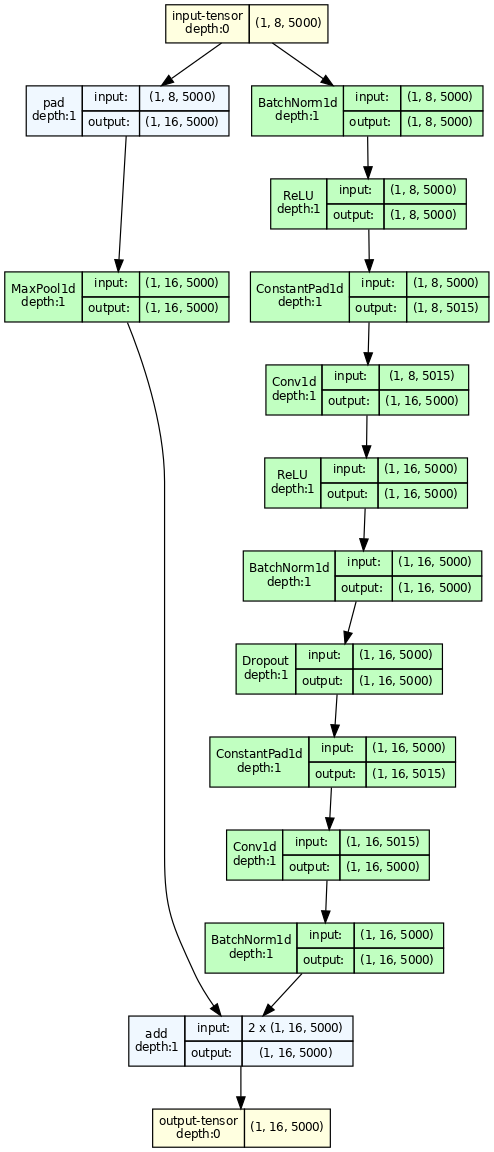
\includegraphics[width=0.65\textwidth]{ResidualMaxPoolDoubleConvBlockForward.gv.png}
	\caption{ResidualMaxPoolDoubleConvBlockForward architecture.}
	\label{fig:resfw_architecture}
\end{figure}

\begin{figure}[p]
	\centering
	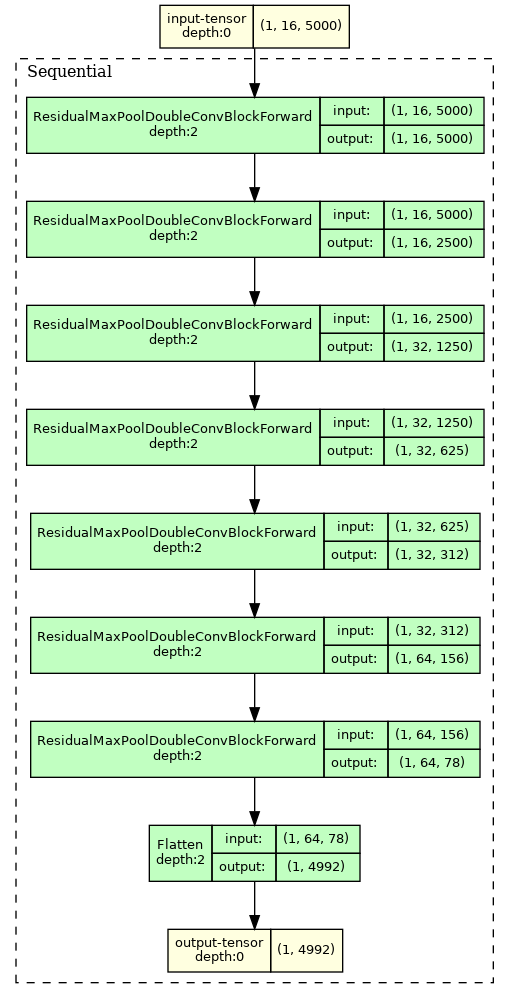
\includegraphics[width=0.7\textwidth]{CNNDoubleResidual.gv.png}
	\caption{CNNDoubleResidual architecture.}
	\label{fig:cnnfw_architecture}
\end{figure}

\begin{figure}[p]
	\centering
	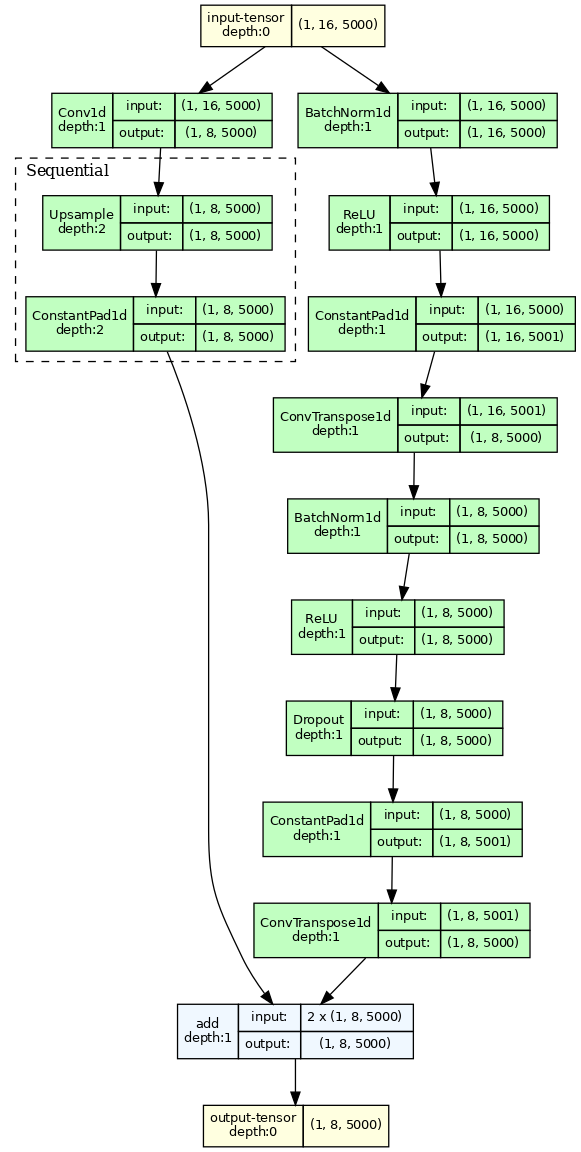
\includegraphics[width=0.7\textwidth]{ResidualMaxPoolDoubleConvBlockBackward.gv.png}
	\caption{ResidualMaxPoolDoubleConvBlockBackward architecture.}
	\label{fig:resbw_architecture}
\end{figure}

\begin{figure}[p]
	\centering
	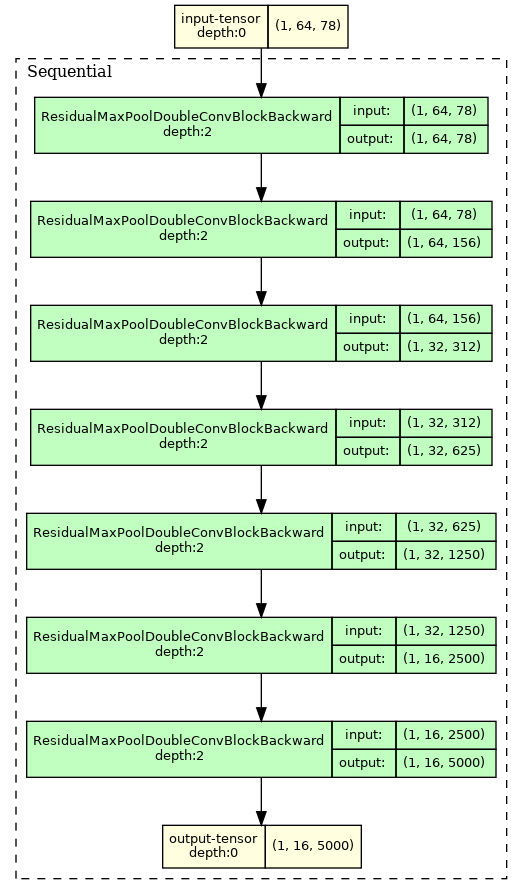
\includegraphics[width=0.7\textwidth]{CNNDoubleResidualBackward.gv.png}
	\caption{CNNDoubleResidualBackward architecture.}
	\label{fig:cnnbw_architecture}
\end{figure}

\begin{figure}[p]
	\makebox[\linewidth][c]{
		\begin{subfigure}[b]{0.6\textwidth}
			\centering
			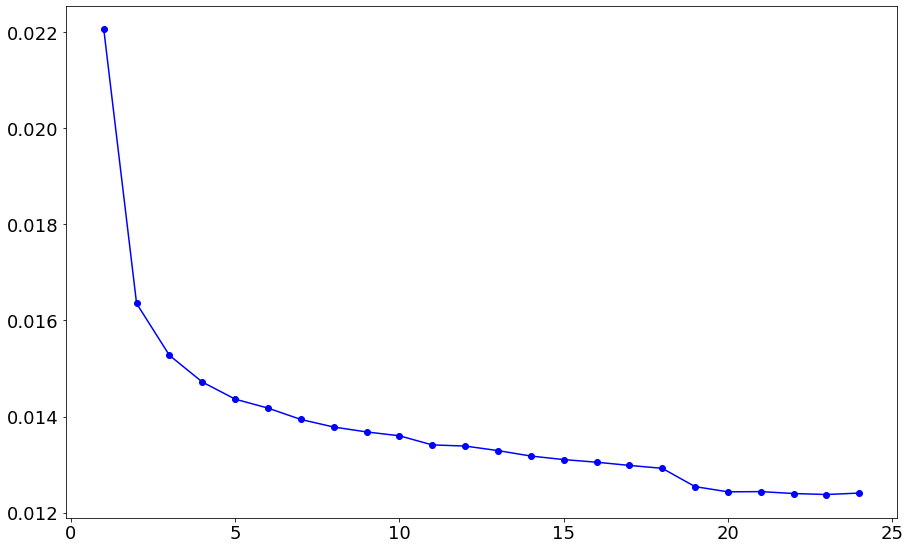
\includegraphics[width=\textwidth]{bc_train_loss.png}
			\caption{Training loss.}
			\label{fig:bc_train_loss}
		\end{subfigure}%
		\begin{subfigure}[b]{0.6\textwidth}
			\centering
			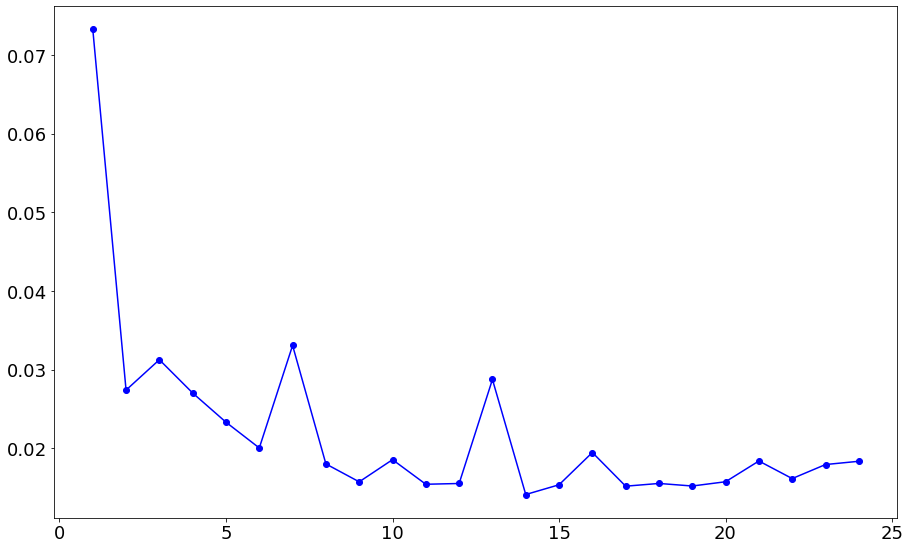
\includegraphics[width=\textwidth]{bc_val_loss.png}
			\caption{Validation loss.}
			\label{fig:bc_val_loss}
		\end{subfigure}
	}
	\vskip\baselineskip
	\makebox[\linewidth][c]{
		\begin{subfigure}[b]{0.6\textwidth}
			\centering
			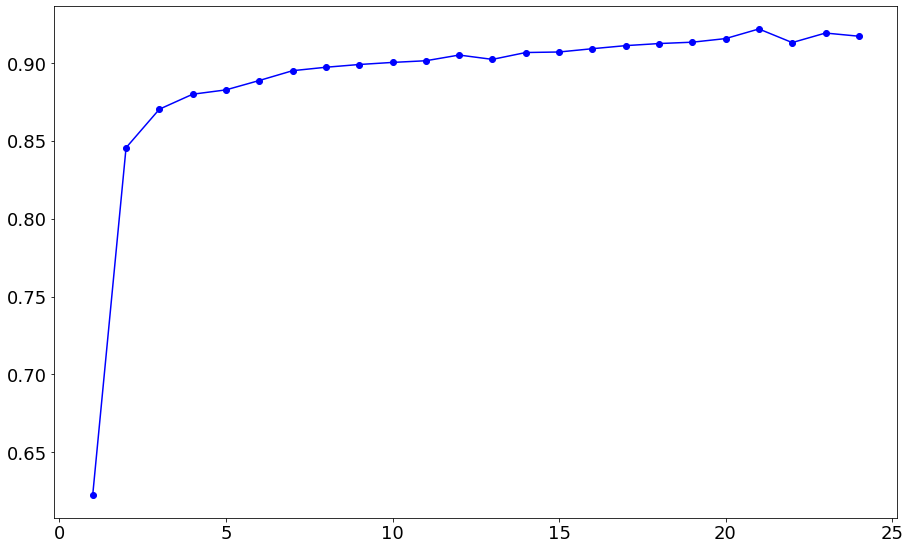
\includegraphics[width=\textwidth]{bc_train_rocauc.png}
			\caption{Training ROC-AUC.}
			\label{fig:bc_train_rocauc}
		\end{subfigure}%
		\begin{subfigure}[b]{0.6\textwidth}
			\centering
			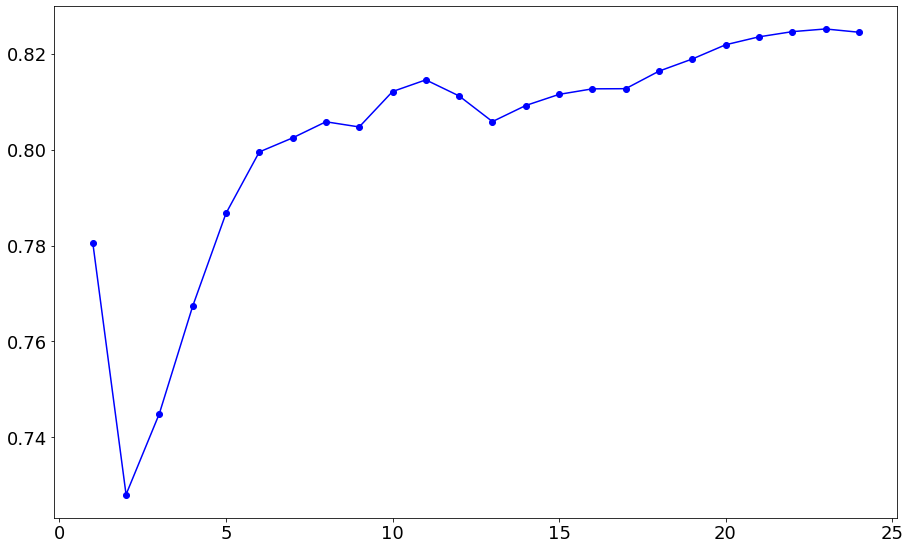
\includegraphics[width=\textwidth]{bc_val_rocauc.png}
			\caption{Validation ROC-AUC.}
			\label{fig:bc_val_rocauc}
		\end{subfigure}
	}
	\caption{Metrics during the training of the BinCl.}
	\label{fig:bc_train_metrics}
\end{figure}

\begin{figure}[H]
	\makebox[\linewidth][c]{
		\centering
		\begin{subfigure}[b]{0.6\textwidth}
			\centering
			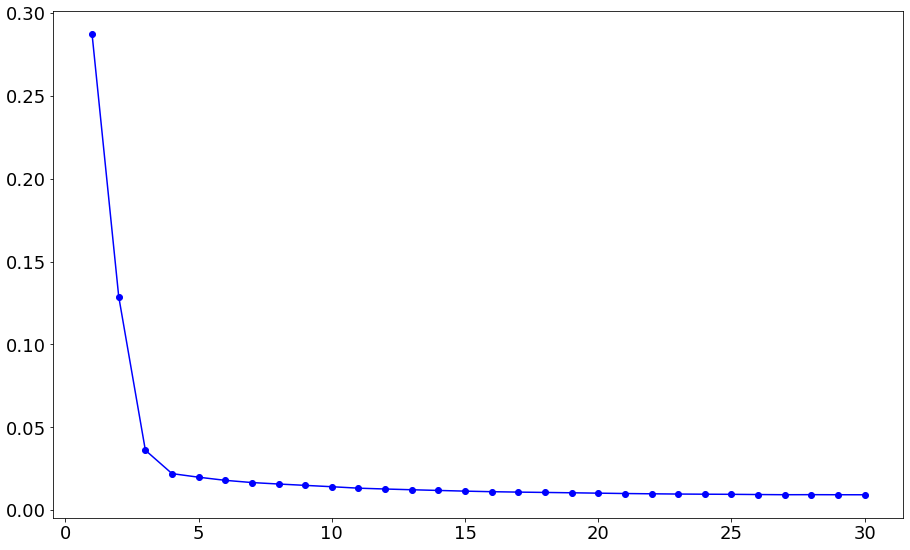
\includegraphics[width=\textwidth]{ae_train_loss.png}
			\caption{Training loss.}
			\label{fig:ae_train_loss}
		\end{subfigure}%
		\begin{subfigure}[b]{0.6\textwidth}
			\centering
			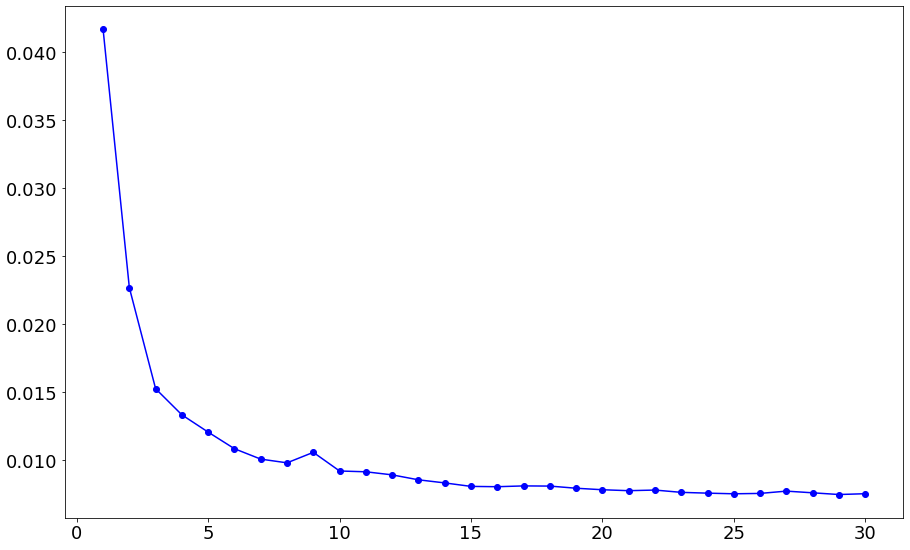
\includegraphics[width=\textwidth]{ae_val_loss.png}
			\caption{Validation loss.}
			\label{fig:ae_val_loss}
		\end{subfigure}
	}
	\caption{Metrics during the training of the AE.}
	\label{fig:ae_metrics}
\end{figure}

\begin{figure}[H]
	\makebox[\linewidth][c]{
		\centering
		\begin{subfigure}[b]{0.6\textwidth}
			\centering
			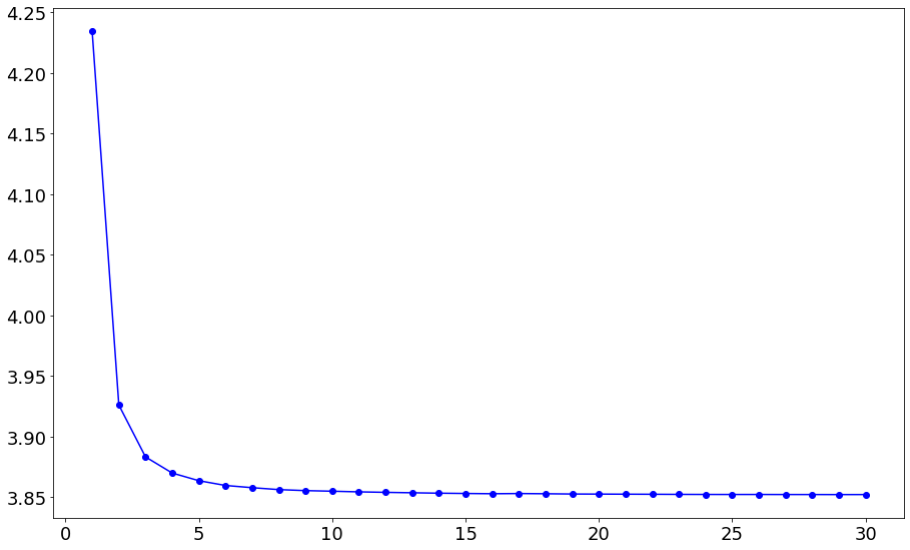
\includegraphics[width=\textwidth]{simclr_train_loss.png}
			\caption{Training loss.}
			\label{fig:simclr_train_loss}
		\end{subfigure}%
		\begin{subfigure}[b]{0.6\textwidth}
			\centering
			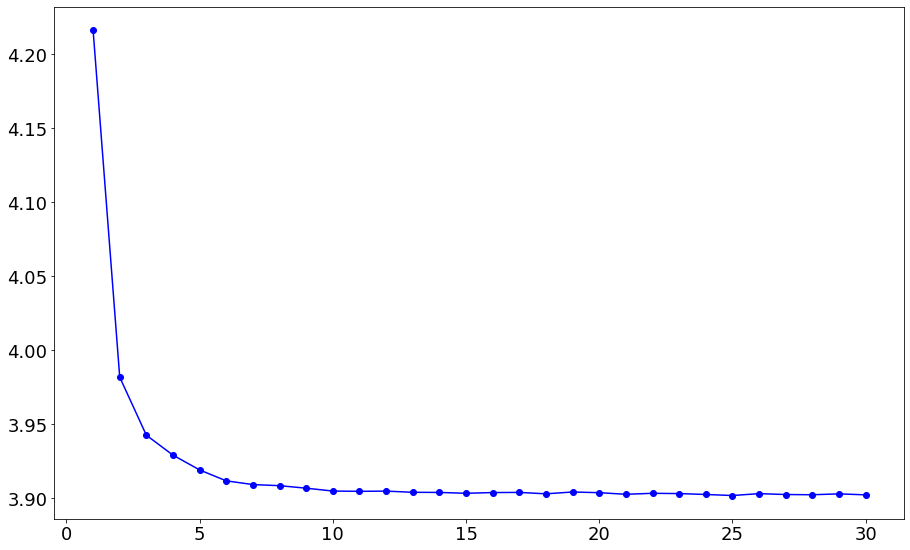
\includegraphics[width=\textwidth]{simclr_val_loss.png}
			\caption{Validation loss.}
			\label{fig:simclr_val_loss}
		\end{subfigure}
	}
	\caption{Metrics during the training of SimCLR.}
	\label{fig:simclr_metrics}
\end{figure}

\begin{figure}[H]
	\centering
	\makebox[\linewidth][c]{
		\begin{subfigure}[b]{0.6\textwidth}
			\centering
			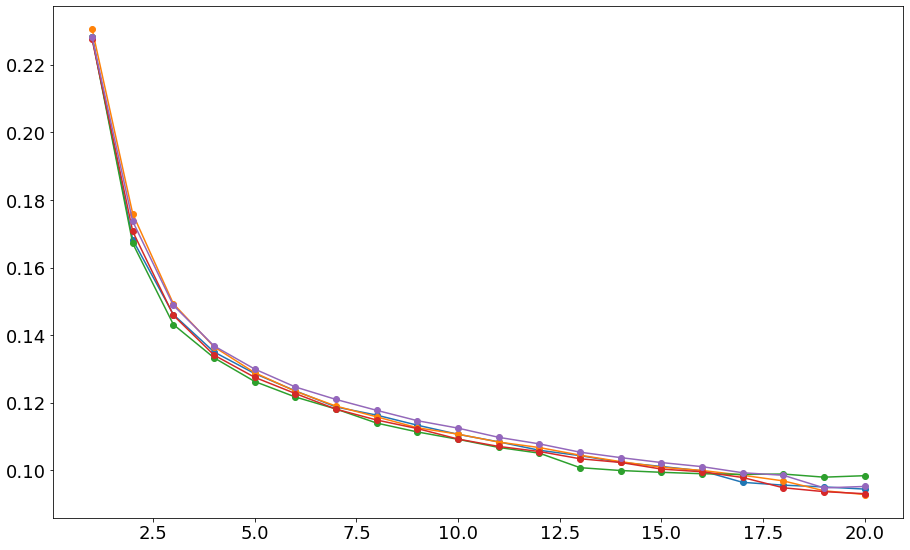
\includegraphics[width=\textwidth]{ens_train_loss.png}
			\caption{Training loss.}
			\label{fig:ens_train_loss}
		\end{subfigure}%
		\begin{subfigure}[b]{0.6\textwidth}
			\centering
			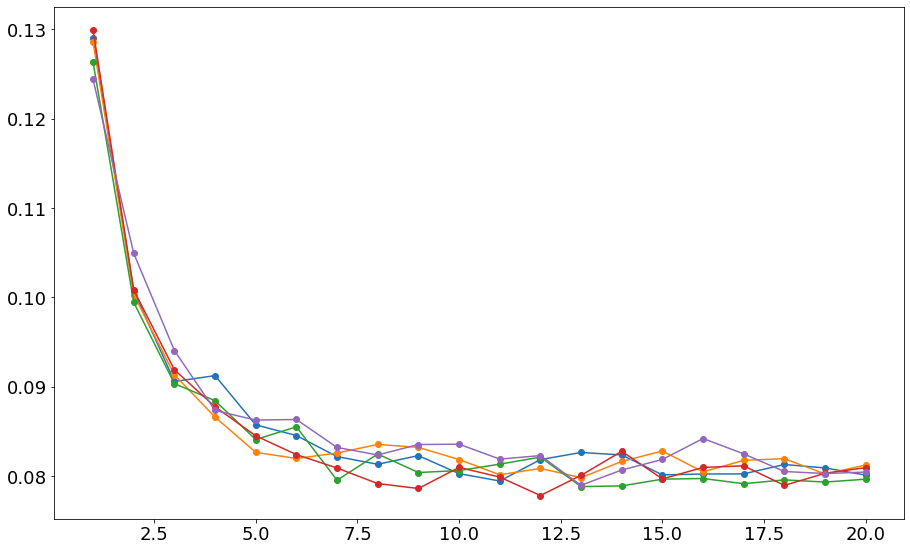
\includegraphics[width=\textwidth]{ens_val_loss.png}
			\caption{Validation loss.}
			\label{fig:ens_val_loss}
		\end{subfigure}
	}
	\caption{Metrics during the training of the DiagCl ensemble.}
	\label{fig:ens_metrics}
\end{figure}

\begin{figure}[p]
	\centering
	\makebox[\linewidth][c]{
		\begin{minipage}{0.6\textwidth}
			\centering
			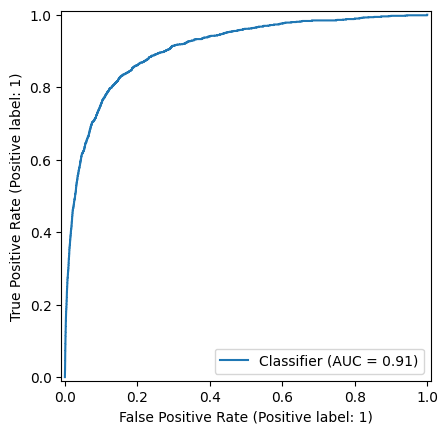
\includegraphics[width=0.9\textwidth]{bincl_umcu_roc.png}
			\caption{BinCl on binary classification data: ROC-AUC curve.}% 
			\label{fig:bincl_umcu_roc}
		\end{minipage}
		\hspace{0.2cm}
		\begin{minipage}{0.6\textwidth}
			\centering
			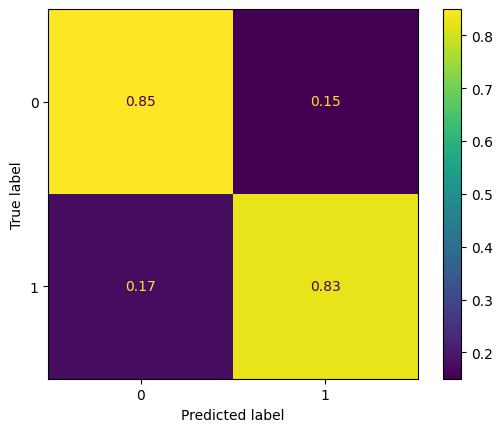
\includegraphics[width=\textwidth]{bincl_umcu_cm.png}
			\caption{BinCl on binary classification data: normalised confusion matrix.}% 
			\label{fig:bincl_umc_cm}
		\end{minipage}
	}
	\vskip5\baselineskip
	\begin{tabular}{r|c|c|c|c}
		                          & \textbf{Precision} & \textbf{Recall} & \textbf{F1-score} & \textbf{Support} \\ \midrule
		\textbf{Clean}            & 0.99               & 0.85            & 0.92              & 37,069           \\
		\textbf{Noisy}            & 0.17               & 0.83            & 0.28              & 1,340            \\ \midrule
		\textbf{Average}          & 0.58               & 0.84            & 0.60              & 38,409           \\
		\textbf{Weighted average} & 0.96               & 0.85            & 0.89              & 38,409
	\end{tabular}
	\captionof{table}{BinCl on binary classification data: classification report.}% 
	\label{tab:bincl_umc_cr}
\end{figure}

\begin{figure}[p]
	\centering
	\makebox[\linewidth][c]{
		\begin{minipage}{0.6\textwidth}
			\centering
			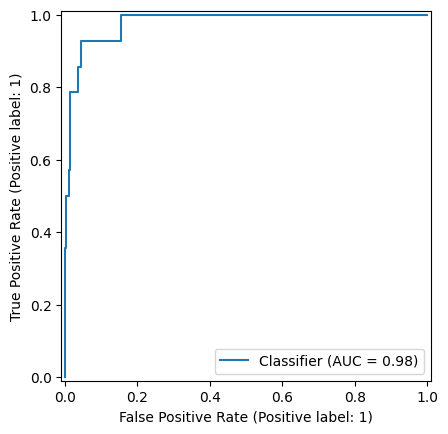
\includegraphics[width=0.9\textwidth]{bincl_segm_roc.png}
			\caption{BinCl on Expert-annotated set: ROC-AUC curve.}% 
			\label{fig:bincl_segm_roc}
		\end{minipage}
		\hspace{0.2cm}
		\begin{minipage}{0.6\textwidth}
			\centering
			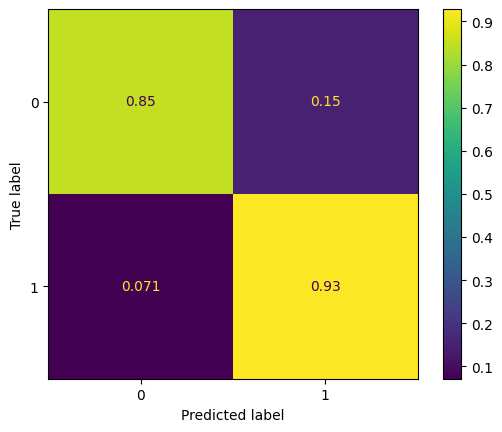
\includegraphics[width=\textwidth]{bincl_segm_cm.png}
			\caption{BinCl on Expert-annotated set: normalised confusion matrix.}% 
			\label{fig:bincl_segm_cm}
		\end{minipage}
	}
	\vskip5\baselineskip
	\centering
	\begin{tabular}{r|c|c|c|c}
		                          & \textbf{Precision} & \textbf{Recall} & \textbf{F1-score} & \textbf{Support} \\ \midrule
		\textbf{Clean}            & 1.00               & 0.74            & 0.85              & 276              \\
		\textbf{Noisy}            & 0.23               & 0.96            & 0.38              & 23               \\ \midrule
		\textbf{Average}          & 0.61               & 0.85            & 0.61              & 299              \\
		\textbf{Weighted average} & 0.94               & 0.76            & 0.81              & 299
	\end{tabular}
	\captionof{table}{BinCl on PhysioNet 2011 data: classification report.}% 
	\label{tab:bincl_segm_cr}
\end{figure}

\begin{figure}[p]
	\centering
	\makebox[\linewidth][c]{
		\begin{minipage}{0.6\textwidth}
			\centering
			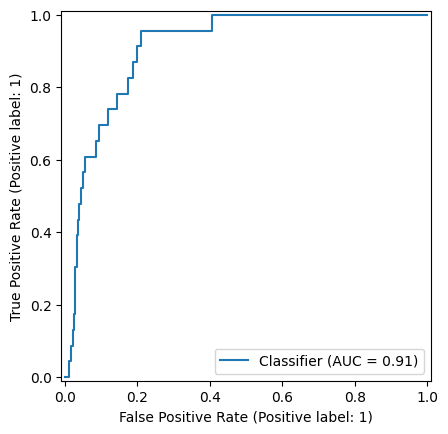
\includegraphics[width=0.9\textwidth]{bincl_phynet_roc.png}
			\caption{BinCl on PhysioNet 2011 data: ROC-AUC curve.}% 
			\label{fig:bincl_phynet_roc}
		\end{minipage}
		\hspace{0.2cm}
		\begin{minipage}{0.6\textwidth}
			\centering
			\includegraphics[width=\textwidth]{bincl_phynet_cm.png}
			\caption{BinCl on PhysioNet 2011 data: normalised confusion matrix.}% 
			\label{fig:bincl_phynet_cm}
		\end{minipage}
	}
	\vskip5\baselineskip
	\begin{tabular}{r|c|c|c|c}
		                          & \textbf{Precision} & \textbf{Recall} & \textbf{F1-score} & \textbf{Support} \\ \midrule
		\textbf{Clean}            & 1.00               & 0.74            & 0.85              & 276              \\
		\textbf{Noisy}            & 0.23               & 0.96            & 0.38              & 23               \\ \midrule
		\textbf{Average}          & 0.61               & 0.85            & 0.61              & 299              \\
		\textbf{Weighted average} & 0.94               & 0.76            & 0.81              & 299
	\end{tabular}
	\captionof{table}{BinCl on PhysioNet 2011 data: classification report.}% 
	\label{tab:bincl_phynet_cr}
\end{figure}

\begin{figure}[p]
	\centering
	\makebox[\linewidth][c]{
		\begin{minipage}{0.6\textwidth}
			\centering
			\includegraphics[width=0.9\textwidth]{ae_split_a_roc.png}
			\caption{AE on Clean split A: ROC-AUC curve.}% 
			\label{fig:ae_clean_a_roc}
		\end{minipage}
		\hspace{0.2cm}
		\begin{minipage}{0.6\textwidth}
			\centering
			\includegraphics[width=\textwidth]{ae_split_a_cm.png}
			\caption{AE on Clean split A: normalised confusion matrix.}
			\label{fig:ae_clean_a_cm}
		\end{minipage}
	}
	\vskip5\baselineskip
	\begin{tabular}{r|c|c|c|c}
		                          & \textbf{Precision} & \textbf{Recall} & \textbf{F1-score} & \textbf{Support} \\ \midrule
		\textbf{Clean}            & 0.85               & 0.72            & 0.78              & 36,593           \\
		\textbf{Noisy}            & 0.43               & 0.63            & 0.51              & 12,612           \\ \midrule
		\textbf{Average}          & 0.64               & 0.67            & 0.65              & 49,205           \\
		\textbf{Weighted average} & 0.74               & 0.70            & 0.71              & 49,205
	\end{tabular}
	\captionof{table}{AE on Clean split A: classification report.}% 
	\label{tab:ae_clean_a_cr}
\end{figure}

\begin{figure}[p]
	\centering
	\makebox[\linewidth][c]{
		\begin{minipage}{0.6\textwidth}
			\centering
			\includegraphics[width=0.9\textwidth]{ae_split_b_roc.png}
			\caption{AE on Clean split B: ROC-AUC curve.}% 
			\label{fig:ae_clean_b_roc}
		\end{minipage}
		\hspace{0.2cm}
		\begin{minipage}{0.6\textwidth}
			\centering
			\includegraphics[width=\textwidth]{ae_split_b_cm.png}
			\caption{AE on Clean split B: normalised confusion matrix.}% 
			\label{fig:ae_clean_b_cm}
		\end{minipage}
	}
	\vskip5\baselineskip
	\begin{tabular}{r|c|c|c|c}
		                          & \textbf{Precision} & \textbf{Recall} & \textbf{F1-score} & \textbf{Support} \\ \midrule
		\textbf{Clean}            & 0.84               & 0.76            & 0.80              & 35,097           \\
		\textbf{Noisy}            & 0.47               & 0.59            & 0.53              & 12,612           \\ \midrule
		\textbf{Average}          & 0.66               & 0.68            & 0.66              & 47,709           \\
		\textbf{Weighted average} & 0.74               & 0.72            & 0.73              & 47,709
	\end{tabular}
	\captionof{table}{AE on Clean split B: classification report.}%
	\label{tab:ae_clean_b_cr}
\end{figure}

\begin{figure}[p]
	\centering
	\makebox[\linewidth][c]{
		\begin{minipage}{0.6\textwidth}
			\centering
			\includegraphics[width=0.9\textwidth]{ae_segm_roc.png}
			\caption{AE on expert-annotated data: ROC-AUC curve.}% 
			\label{fig:ae_segm_roc}
		\end{minipage}
		\hspace{0.2cm}
		\begin{minipage}{0.6\textwidth}
			\centering
			\includegraphics[width=\textwidth]{ae_split_b_cm.png}
			\caption{AE on expert-annotated data: normalised confusion matrix.}% 
			\label{fig:ae_segm_cm}
		\end{minipage}
	}
	\vskip5\baselineskip
	\begin{tabular}{r|c|c|c|c}
		                          & \textbf{Precision} & \textbf{Recall} & \textbf{F1-score} & \textbf{Support} \\ \midrule
		\textbf{Clean}            & 0.99               & 0.71            & 0.83              & 962              \\
		\textbf{Noisy}            & 0.03               & 0.64            & 0.06              & 14               \\ \midrule
		\textbf{Average}          & 0.51               & 0.68            & 0.44              & 976              \\
		\textbf{Weighted average} & 0.98               & 0.71            & 0.82              & 976
	\end{tabular}
	\captionof{table}{AE on expert-annotated data: classification report.}%
	\label{tab:ae_segm_cr}
\end{figure}

\begin{figure}[p]
	\centering
	\makebox[\linewidth][c]{
		\begin{minipage}{0.6\textwidth}
			\centering
			\includegraphics[width=0.9\textwidth]{ae_phynet_roc.png}
			\caption{AE on PhysioNet 2011: ROC-AUC curve.}% 
			\label{fig:ae_phynet_roc}
		\end{minipage}
		\hspace{0.2cm}
		\begin{minipage}{0.6\textwidth}
			\centering
			\includegraphics[width=\textwidth]{ae_split_b_cm.png}
			\caption{AE on PhysioNet 2011: normalised confusion matrix.}% 
			\label{fig:ae_phynet_cm}
		\end{minipage}
	}
	\vskip5\baselineskip
	\begin{tabular}{r|c|c|c|c}
		\multicolumn{1}{l|}{}     & \textbf{Precision} & \textbf{Recall} & \textbf{F1-score} & \textbf{Support} \\ \midrule
		\textbf{Clean}            & 1.00               & 0.78            & 0.87              & 276              \\
		\textbf{Noisy}            & 0.26               & 0.96            & 0.41              & 23               \\ \midrule
		\textbf{Average}          & 0.63               & 0.87            & 0.64              & 299              \\
		\textbf{Weighted average} & 0.94               & 0.79            & 0.84              & 299
	\end{tabular}
	\captionof{table}{AE on PhysioNet 2011: classification report.}%
	\label{tab:ae_phynet_cr}
\end{figure}

\begin{figure}[p]
	\centering
	\makebox[\linewidth][c]{
		\begin{minipage}{0.6\textwidth}
			\centering
			\includegraphics[width=0.9\textwidth]{feature_phynet_roc.png}
			\caption{SimCLR for feature clustering on PhysioNet 2011: ROC-AUC curve.}% 
			\label{fig:feature_phynet_roc}
		\end{minipage}
		\hspace{0.2cm}
		\begin{minipage}{0.6\textwidth}
			\centering
			\includegraphics[width=\textwidth]{feature_phynet_cm.png}
			\caption{AE on PhysioNet 2011: normalised confusion matrix.}% 
			\label{fig:feature_phynet_cm}
		\end{minipage}
	}
	\vskip5\baselineskip
	\begin{tabular}{r|c|c|c|c}
		                          & \textbf{Precision} & \textbf{Recall} & \textbf{F1-score} & \textbf{Support} \\ \midrule
		\textbf{Clean}            & 1.00               & 0.81            & 0.89              & 276              \\
		\textbf{Noisy}            & 0.29               & 0.96            & 0.45              & 23               \\ \midrule
		\textbf{Average}          & 0.64               & 0.88            & 0.67              & 299              \\
		\textbf{Weighted average} & 0.94               & 0.82            & 0.86              & 299
	\end{tabular}
	\captionof{table}{SimCLR for feature clustering on PhysioNet 2011: classification report.}
	\label{tab:feature_phynet_cr}
\end{figure}

\begin{figure}[p]
	\makebox[\linewidth][c]{
		\begin{minipage}{1.2\textwidth}
			\centering
			\includegraphics[width=\textwidth]{diagcl_rhythm_cm.png}
			\caption{DiagCl ensemble, Rhythm Type labels: confusion matrix.}
			\label{fig:diagcl_rhythm_cm}
		\end{minipage}
	}
\end{figure}

\begin{figure}[p]
	\begin{minipage}{\textwidth}
		\centering
		\includegraphics[width=0.8\textwidth]{diagcl_avc_cm.png}
		\caption{DiagCl ensemble, AVC labels: confusion matrix.}
		\label{fig:diagcl_avc_cm}
	\end{minipage}
	\vskip2\baselineskip
	\begin{minipage}{\textwidth}
		\centering
		\includegraphics[width=0.8\textwidth]{diagcl_vc_cm.png}
		\caption{DiagCl ensemble, VC labels: confusion matrix.}
		\label{fig:diagcl_vc_cm}
	\end{minipage}
\end{figure}

\begin{figure}[p]
	\centering
	\begin{minipage}{\textwidth}
		\centering
		\includegraphics[width=0.8\textwidth]{diagcl_ischemia_cm.png}
		\caption{DiagCl ensemble, Ischemia labels: confusion matrix.}
		\label{fig:diagcl_ischemia_cm}
	\end{minipage}
	\vskip5\baselineskip
	\begin{tabular}{r|c}
		\textbf{Condition} & \textbf{ROC-AUC}   \\ \midrule
		oldischemia        & 0.8713090894371586 \\
		other\_lvh         & 0.9444848639303637 \\
		other\_pc          & 0.9456560317017403 \\
		rhythm\_wpw        & 0.980714054299229  \\
		qrs\_pvc           & 0.9618043914938221 \\
		rhythm\_pac        & 0.8929069326422576
	\end{tabular}
	\captionof{table}{DiagCl ensemble, Other labels: ROC-AUC.}
	\label{tab:diag_other_roc-auc}
\end{figure}

\end{document}